%% Dokumentenklasse (Koma Script)
\documentclass[%
   %draft,     % Entwurfsstadium
   final,      % fertiges Dokument
%%%% --- Schriftgröße ---
   11pt,
%%%% --- Sprache ---
   english,
   ngerman,           % Letzte Sprache ist die Hauptsprache, andere muss erst ausgewählt werden.
%%%% === Seitengröße ===
   a4paper,
%%%% === Optionen für den Satzspiegel ===
   %BCOR5mm,         % Zusaetzlicher Rand auf der Innenseite (Bindekorrektur)
   %DIV11,           % Seitengroesse (siehe Koma Skript Dokumentation!)
   %DIVcalc,         % automatische Berechnung einer guten Zeilenlaenge
   1.1headlines,     % Zeilenanzahl der Kopfzeilen
   %headinclude,     % Kopf einbeziehen
   headinclude=false,      % Kopf nicht einbeziehen
   %footinclude,     % Fuss einbeziehen
   footinclude=false,      % Fuss nicht einbeziehen
   %mpinclude,       % Margin einbeziehen
   mpinclude=false,        % Margin nicht einbeziehen
   pagesize,         % Schreibt die Papiergroesse in die Datei.
                     % Wichtig fuer Konvertierungen
%%%% === Layout ===
   %oneside,          % einseitiges Layout
   twoside,         % Seitenraender für zweiseitiges Layout
   onecolumn,        % Einspaltig
   %twocolumn,       % Zweispaltig
   %openany,         % Kapitel beginnen auf jeder Seite
   %openright,        % Kapitel beginnen immer auf der rechten Seite
                     % (macht nur bei 'twoside' Sinn)
   %cleardoubleplain,    % leere, linke Seite mit Seitenstil 'plain'
   %cleardoubleempty,    % leere, linke Seite mit Seitenstil 'empty'
   titlepage,        % Titel als einzelne Seite ('titlepage' Umgebung)
   %notitlepage,     % Titel in Seite integriert
%%%% --- Absatzeinzug ---
   %                 % Absatzabstand: Einzeilig,
   %parskip,         % Freiraum in letzter Zeile: 1em
   %parskip*,        % Freiraum in letzter Zeile: Viertel einer Zeile
   %parskip+,        % Freiraum in letzter Zeile: Drittel einer Zeile
   %parskip-,        % Freiraum in letzter Zeile: keine Vorkehrungen
   %                 % Absatzabstand: Halbzeilig
   %halfparskip,     % Freiraum in letzter Zeile: 1em
   %halfparskip*,    % Freiraum in letzter Zeile: Viertel einer Zeile
   %halfparskip+,    % Freiraum in letzter Zeile: Drittel einer Zeile
   parskip=half,      % Freiraum in letzter Zeile: keine Vorkehrungen
   %                 % Absatzabstand: keiner
   %parindent,       % Eingerückt (Standard)
%%%% --- Kolumnentitel ---
   headsepline,      % Linie unter Kolumnentitel
   %headnosepline,   % keine Linie unter Kolumnentitel
   %footsepline,     % Linie unter Fussnote
   %footnosepline,   % keine Linie unter Fussnote
%%%% --- Kapitel ---
   %chapterprefix,   % Ausgabe von 'Kapitel:'
   chapterprefix=false,
   version=first,  % keine Ausgabe von 'Kapitel:'
%%%% === Verzeichnisse (TOC, LOF, LOT, BIB) ===
   listof=totoc,      % Tabellen & Abbildungsverzeichnis ins TOC
   %idxtotoc,        % Index ins TOC
   bibliography=totoc,
   verson=first,         % Bibliographie ins TOC
   %bibtotocnumbered, % Bibliographie im TOC nummeriert
   %liststotocnumbered, % Alle Verzeichnisse im TOC nummeriert
   toc=graduated,        % eingereuckte Gliederung
   %tocleft,         % Tabellenartige TOC
   %listsindent,      % eingereuckte LOT, LOF
   %listsleft,       % Tabellenartige LOT, LOF
   %pointednumbers,  % Überschriftnummerierung mit Punkt, siehe DUDEN !
   %pointlessnumbers, % Überschriftnummerierung ohne Punkt, siehe DUDEN !
   %openbib,         % alternative Formatierung des Literaturverzeichnisses
%%%% === Matheformeln ===
   %leqno,           % Formelnummern links
   fleqn,            % Formeln werden linksbuendig angezeigt
]{scrbook}%     Klassen: scrartcl, scrreprt, scrbook
% -------------------------------------------------------------------------

% -------------- Daten für die Titelseite --> diese müssen angepasst werden!
\newcommand*{\thedockind}{Bachelorthesis}
\newcommand*{\thetitle}{Verl{\"a}ssliche mobile Anwendungen}
\newcommand*{\thesubtitle}{Untersuchungen am Beispiel einer Fitness-App}
\newcommand*{\theauthor}{Kevin Schie / Stefan Suermann}
\newcommand*{\thematriculationnumber}{2012013 / 2012027} % Matrikelnummer
\newcommand*{\thebirthday}{04.07.1993 / 13.12.1987} % Geburtstag
\newcommand*{\thedegree}{Bachelor of Science}
\newcommand*{\themajor}{IT- und Softwaresysteme} % Studiengang
\newcommand*{\thedate}{\today} % \today kann durch ein Datum erstetzt werden.
\newcommand*{\thebetreuer}{Prof. Dr. Johannes Ecke-Sch{\"u}th}
\newcommand*{\thezweitbetreuer}{Prof. Dr. Klaus-Dieter Kr{\"a}geloh}
% -------------- Ende Daten für die Titelseite

%%% Doc: ftp://tug.ctan.org/pub/tex-archive/macros/latex/required/babel/babel.pdf
% Languagesetting
\usepackage{babel}	% Sprache

\usepackage{textpos} 


\usepackage{fixltx2e}	% Verbessert einige Kernkompetenzen von LaTeX2e
\usepackage{ellipsis}	% Korrigiert den Wei�raum um Auslassungspunkte

\usepackage{placeins} 

\usepackage{ifpdf}
\ifpdf
\pdfinfo {
	/Author (\theauthor)
	/Title (\thetitle)
	/Subject ()
	/Keywords ()
%	/CreationDate (D:YYYYMMTTHHMMSS)
}
\fi



%%% Doc: www.cs.brown.edu/system/software/latex/doc/calc.pdf
% Calculation with LaTeX
\usepackage{calc}

%%% Doc: ftp://tug.ctan.org/pub/tex-archive/macros/latex/contrib/xcolor/xcolor.pdf
% Farben
% Incompatible: Do not load when using pstricks !
\usepackage[
	table % Load for using rowcolors command in tables
]{xcolor}

\usepackage{tikz}
\usetikzlibrary{% 
   arrows,% 
   calc,% 
   fit,% 
   patterns,% 
   plotmarks,% 
   shapes.geometric,% 
   shapes.misc,% 
   shapes.symbols,% 
   shapes.arrows,% 
   shapes.callouts,% 
   shapes.multipart,% 
   shapes.gates.logic.US,% 
   shapes.gates.logic.IEC,% 
   er,% 
   automata,% 
   backgrounds,% 
   chains,% 
   topaths,% 
   trees,% 
   petri,% 
   mindmap,% 
   matrix,% 
   calendar,% 
   folding,% 
   fadings,% 
   through,% 
   positioning,% 
   scopes,% 
   decorations.fractals,% 
   decorations.shapes,% 
   decorations.text,% 
   decorations.pathmorphing,% 
   decorations.pathreplacing,% 
   decorations.footprints,% 
   decorations.markings,% 
   shadows} 
   
%%% Doc: ftp://tug.ctan.org/pub/tex-archive/macros/latex/required/graphics/grfguide.pdf
% Bilder
\usepackage[%
	%final,
	%draft % do not include images (faster)
]{graphicx}


% bessere Abstaende innerhalb der Tabelle (Layout))
% -------------------------------------------------
%%% Doc: ftp://tug.ctan.org/pub/tex-archive/macros/latex/contrib/booktabs/booktabs.pdf
\usepackage{booktabs}


%%% Doc: ftp://tug.ctan.org/pub/tex-archive/macros/latex/contrib/enumitem/enumitem.pdf
% Better than 'paralist' and 'enumerate' because it uses a keyvalue interface!
% Do not load together with enumerate.
%\usepackage{enumitem}

\usepackage{paralist}


%%% Doc: http://www.ctan.org/tex-archive/macros/latex/contrib/acronym/acronym.pdf
% Usage:
%        Definition: \acro{ acronym }[ short name ]{ full name }
%        Nutzung im Text: \ac{acronym}
 \usepackage[
 	%footnote,	% Full names appear in the footnote
 	%smaller,		% Print acronym in smaller fontsize
 	%printonlyused %
 ]{acronym}
%\chapter*{Abkürzungsverzeichnis}
\addcontentsline{toc}{chapter}{Abkürzungsverzeichnis}  
\begin{acronym}[Visual Studio] %Längster Begriff
\setlength{\itemsep}{-\parsep}
	\acro{.apk}{Android Package}
	\acro{ACL}{Access Control Lists}
	\acro{AES}{Advanced Encryption Standard}
	\acro{AJAX}{Asynchronous JavaScript and XML}	
	\acro{ANR}{Application Not Responding}
	\acro{API}{Application Programming Interface}
	\acro{CORS}{Cross-origin resource sharing}
	\acro{CRUD}{Create Read Update Delete}	
	\acro{CSS}{Cascading Style Sheet}
	\acro{DLL}{Dynamic Link Library}
	\acro{DRAM}{Dynamischer \ac{RAM}}
	\acro{HTML}{Hypertext Markup Language}	
	\acro{HTTP}{Hypertext Transfer Protocol}	
	\acro{HTTPS}{Hyper Text Transfer Protocol Secure}	
	\acro{IDE}{Integrated Development Environment}
	\acro{JSON}{JavaScript Object Notation}	
	\acro{JWT}{\ac{JSON} Web Token}	
	\acro{MSSQL}{Microsoft SQL Server}
	\acro{MVC}{Model-View-Controller}	
	\acro{MVVM}{Model-View-ViewModel}
	\acro{OR-Mapper}{objekt-relationaler Mapper}
	\acro{PCL}{Portable Class Library}
	\acro{RAM}{Random Access Memory}
	\acro{RBAC}{Role Based Access Control}	
	\acro{REST}{Representational State Transfer}	
	\acro{SPA}{Single Page Application}
	\acro{SRAM}{Statischer \ac{RAM}}
	\acro{TCP}{Transmission Control Protocol}
	\acro{URI}{Uniform Resource Identifier}		
	\acro{URL}{Uniform Resource Locator}		
	\acro{Visual Studio}{Microsoft Visual Studio 2015 Community Edition}		
	\acro{VM}{Virtuelle Maschine}
	\acro{Web-App}{mobil-optimierte Webseite}
	\acro{XML}{Extensible Markup Language}
\end{acronym}



%% Kopf und Fusszeilen====================================================
%%% Doc: ftp://tug.ctan.org/pub/tex-archive/macros/latex/contrib/koma-script/scrguide.pdf
\usepackage[%
   automark,         % automatische Aktualisierung der Kolumnentitel
   %nouppercase,      % Grossbuchstaben verhindern
   %markuppercase    % Grossbuchstaben erzwingen
   %markusedcase     % vordefinierten Stil beibehalten
   %komastyle,       % Stil von Koma Script
   %standardstyle,   % Stil der Standardklassen
]{scrpage2}



%% UeberSchriften (Chapter und Sections) =================================
% -- Ueberschriften komlett Umdefinieren --
%%% Doc: ftp://tug.ctan.org/pub/tex-archive/macros/latex/contrib/titlesec/titlesec.pdf
\usepackage{titlesec}

% -- Section Aussehen veraendern --
% --------------------------------
%% -> Section mit Unterstrich
% \titleformat{\section}
%   [hang]%[frame]display
%   {\usekomafont{sectioning}\Large}
%  {\thesection}
%   {6pt}
%   {}
%   [\titlerule \vspace{0.5\baselineskip}]
% --------------------------------

% -- Chapter Aussehen veraendern --
% --------------------------------
\titleformat{\chapter}[block]	% {command}[shape]
  {\usekomafont{chapter}\huge\sffamily\bfseries}	% format
  {   										% label
  {\thechapter.} \filright%
  }%}
  {1pt}										% sep (from chapternumber)
  {\vspace{0.5pc} \filright}   % {before}[after] (before chaptertitle and after)
  [\vspace{0.5pc} \filright {}]

% \titleformat{\chapter}[]%
%    {\usekomafont{chapter}\huge\sffamily\bfseries}%
%    {\thechapter}%
%    {1em}%
%    {}%


\usepackage{rotating}

%Literatur-Einstellungen

%vielleicht Layout anpassen...

\usepackage[%
style=authortitle-dw,
namefont=smallcaps,%
firstnamefont=smallcaps,%
idemfont=smallcaps,% Schriftart von »Ders.« / »Dies.«
%ibidemfont=smallcaps,% Schriftart von »ebenda« / »ebd.«
idembib=true,% aufeinanderfolgende Einträge -> »Ders.« bzw. »Dies.«
idembibformat=idem,% idem= Ders./Dies.; alternativ: =dash macht Strich -
edbyidem=true,% Autor und Herausgeber bei @incollection- oder @inbook- Einträgen dieselben
nopublisher=true,% true unterdrückt den Verlag
%nolocation=true,% true unterdrückt den Ort, dito doi=true, eprint=true, isbn=true bzw. issn=true
backend=bibtex,
useeditor=true,% Herausgeber vor dem Buchtitel
firstfull=false,% Erste Erwähnung nicht als Vollzitat
shorthandwidth=3em,% Breite der Label im Sigelverzeichnis angeben.
%firstinits=,% Initialen der Vornamen
%uniquename=init,% Gibt bei Autoren mit gleichem Nachnamen die Initialen mit aus
]{biblatex} 
\DeclareNameFormat{sortname}{% Reihenfolge Nachname Vorname Bibliographie
\iffirstinits
{\usebibmacro{name:last-first}{#1}{#4}{#5}{#7}}
{\usebibmacro{name:last-first}{#1}{#3}{#5}{#7}}%
\usebibmacro{name:andothers}}

\bibliography{bib/bib}

\renewbibmacro*{author/editor/translator}{%
\ifthenelse{\ifuseauthor\AND\NOT\ifnameundef{author}}
{\usebibmacro{author}\addspace(\printfield{shorttitle})}
{\ifthenelse{\ifuseeditor\AND\NOT\ifnameundef{editor}}
{\usebibmacro{editor}\addspace(\printfield{shorttitle})}
{\usebibmacro{translator}\addspace(\printfield{shorttitle})}}}


%Kurzzitat-Schreibweise



% Quotes =================================================================
%% Doc: ftp://tug.ctan.org/pub/tex-archive/macros/latex/contrib/csquotes/csquotes.pdf
% Advanced features for clever quotations
\usepackage[%
   babel,            % the style of all quotation marks will be adapted
                     % to the document language as chosen by 'babel'
   german=quotes,		% Styles of quotes in each language
   %german=guillemets,
   english=british,
   french=guillemets
]{csquotes}
\usepackage{floatflt}

\usepackage{wrapfig}

%\usepackage{subfigure}

\usepackage{blindtext}

\usepackage{listings}
\definecolor{lila}{RGB}{112, 6, 147}
\definecolor{kommentgreen}{RGB}{5,132,71}
\definecolor{grey}{RGB}{242,242,242}  
\definecolor{darkgreen}{named}{green}
\definecolor{darkblue}{named}{blue}
\definecolor{lightblue}{RGB} {63,95,191}
\definecolor{darkred}{named}{red}
\definecolor{grau}{named}{gray}
\definecolor{fh_orange}{rgb}{0.953,0.201,0}
\definecolor{fh_grau}{rgb}{0.76,0.75,0.76}
\definecolor{lightgray}{rgb}{0.95, 0.95, 0.95}
\definecolor{darkgray}{rgb}{0.4, 0.4, 0.4}
\definecolor{editorGray}{rgb}{0.95, 0.95, 0.95}
\definecolor{editorOcher}{rgb}{1, 0.5, 0} % #FF7F00 -> rgb(239, 169, 0)
\definecolor{editorGreen}{rgb}{0, 0.5, 0} % #007C00 -> rgb(0, 124, 0)
\definecolor{orange}{rgb}{1,0.45,0.13}		
\definecolor{olive}{rgb}{0.17,0.59,0.20}
\definecolor{brown}{rgb}{0.69,0.31,0.31}
\definecolor{purple}{rgb}{0.38,0.18,0.81}
\definecolor{lightblue}{rgb}{0.1,0.57,0.7}
\definecolor{lightred}{rgb}{1,0.4,0.5}

\definecolor{listinggray}{gray}{0.9}
\definecolor{lbcolor}{rgb}{0.9,0.9,0.9}

\lstset{
	tabsize=3,
	float=tbph,
	frame=single,
	extendedchars,
	breaklines=true,
	basicstyle=\fontsize{9pt}{9pt}\selectfont,
	columns=flexible, %ist notwendig, damit man Quelltext aus den Listings kopieren kann
	numbers=left, 
	numberstyle=\color{black},
	captionpos=b,
	aboveskip=7mm,
	backgroundcolor=\color{grey}
}

\lstdefinestyle{java}
{
	language=Java,
	keywordstyle=\color{lila},  	% underlined bold black keywords 
	identifierstyle=\color{blue}, 
	commentstyle=\color{kommentgreen}, % white comments 
	stringstyle=\color{black},
}

\lstdefinelanguage{CSS}{
  keywords={color,background-image:,margin,padding,font,weight,display,position,top,left,right,bottom,list,style,border,size,white,space,min,width, transition:, transform:, transition-property, transition-duration, transition-timing-function},	
  sensitive=true,
  morecomment=[l]{//},
  morecomment=[s]{/*}{*/},
  morestring=[b]',
  morestring=[b]",
  alsoletter={:},
  alsodigit={-}
}

% JavaScript
\lstdefinelanguage{JavaScript}{
  morekeywords={typeof, new, true, false, catch, function, return, null, catch, switch, var, if, in, while, do, else, case, break},
  morecomment=[s]{/*}{*/},
  morecomment=[l]//,
  morestring=[b]",
  morestring=[b]'
}

\lstdefinelanguage{HTML5}{
  language=html,
  sensitive=true,	
  alsoletter={<>=-},	
  morecomment=[s]{<!-}{-->},
  tag=[s],
  otherkeywords={
  % General
  >,
  % Standard tags
	<!DOCTYPE,
  </html, <html, <head, <title, </title, <style, </style, <link, </head, <meta, />,
	% body
	</body, <body,
	% Divs
	</div, <div, </div>, 
	% Paragraphs
	</p, <p, </p>,
	% scripts
	</script, <script,
  % More tags...
  <canvas, /canvas>, <svg, <rect, <animateTransform, </rect>, </svg>, <video, <source, <iframe, </iframe>, </video>, <image, </image>, <header, </header, <article, </article, </nav, <nav, <ul, </ul, <span, </span, <li, </li, <a, </a
  },
  ndkeywords={
  % General
  =,
  % HTML attributes
  charset=, src=, id=, width=, height=, style=, type=, rel=, href=, class=, role=
  % SVG attributes
  fill=, attributeName=, begin=, dur=, from=, to=, poster=, controls=, x=, y=, repeatCount=, xlink:href=,
  % properties
  margin:, padding:, background-image:, border:, top:, left:, position:, width:, height:, margin-top:, margin-bottom:, font-size:, line-height:,
	% CSS3 properties
  transform:, -moz-transform:, -webkit-transform:,
  animation:, -webkit-animation:,
  transition:,  transition-duration:, transition-property:, transition-timing-function:,
  }
}

\lstdefinestyle{htmlcssjs} {%
  % General design
%  backgroundcolor=\color{editorGray},
  basicstyle={\footnotesize\ttfamily},   
  frame=b,
  % line-numbers
  xleftmargin={0.75cm},
  numbers=left,
  stepnumber=1,
  firstnumber=1,
  numberfirstline=true,	
  % Code design
  identifierstyle=\color{black},
  keywordstyle=\color{blue}\bfseries,
  ndkeywordstyle=\color{editorGreen}\bfseries,
  stringstyle=\color{editorOcher}\ttfamily,
  commentstyle=\color{brown}\ttfamily,
  % Code
  language=HTML5,
  alsolanguage=JavaScript,
  alsodigit={.:;},	
  tabsize=2,
  showtabs=false,
  showspaces=false,
  showstringspaces=false,
  extendedchars=true,
  breaklines=true,  
  escapechar=|,
  % German umlauts
  literate=%
  {Ö}{{\"O}}1
  {Ä}{{\"A}}1
  {Ü}{{\"U}}1
  {ß}{{\ss}}1
  {ü}{{\"u}}1
  {ä}{{\"a}}1
  {ö}{{\"o}}1
}
\lstdefinestyle{xml}
{
	language=xml,
	basicstyle=\fontsize{9pt}{9pt}\selectfont\color{kommentgreen},
	keywordstyle=\color{lila},  	% underlined bold black keywords 
	%Hier können bei Bedarf noch weitere Keywords eingetragen werden
	keywords={name, value, version, encoding, id, type, xmlns:xsi, ref, namespace},
	identifierstyle=\color{black},  
	stringstyle=\color{blue},  
	commentstyle=\color{lightblue},
	morecomment=[s]{<!--}{-->},
	rulecolor=\color{black}
}


\definecolor{bluekeywords}{rgb}{0,0,1}
\definecolor{greencomments}{rgb}{0,0.5,0}
\definecolor{redstrings}{rgb}{0.64,0.08,0.08}
\definecolor{xmlcomments}{rgb}{0.5,0.5,0.5}
\definecolor{types}{rgb}{0.17,0.57,0.68}

\lstdefinestyle{sharpc}{
language=[Sharp]C, 
frame=lines, % Oberhalb und unterhalb des Listings ist eine Linie
showspaces=false,
showtabs=false,
breaklines=true,
showstringspaces=false,
breakatwhitespace=true,
escapeinside={(*@}{@*)},
commentstyle=\color{greencomments},
morekeywords={partial, var, value, get, set},
keywordstyle=\color{bluekeywords},
stringstyle=\color{redstrings},
basicstyle=\ttfamily\small,
escapechar=|
}

\definecolor{lightgray}{rgb}{.9,.9,.9}
\definecolor{darkgray}{rgb}{.4,.4,.4}
\definecolor{purple}{rgb}{0.65, 0.12, 0.82}

\usepackage{multicol}

\usepackage{nameref}

\usepackage{hyperref}
\hypersetup{breaklinks=true}
\hypersetup{colorlinks=true,linkcolor=black,urlcolor=black,citecolor=black}
%\hypersetup{frenchlinks}	% Use small caps instead of color for links
%\hypersetup{pdfpagemode=FullScreen}
%\hypersetup{pdfstartpage=3}
%\hypersetup{pdfstartview=Fit}


% Tabellen ueber mehere Seiten
% ----------------------------
%%% Doc: ftp://tug.ctan.org/pub/tex-archive/macros/latex/contrib/carlisle/ltxtable.pdf
% \usepackage{ltxtable} % Longtable + tabularx
                        % (multi-page tables) + (auto-sized columns in a fixed width table)
% -> nach hyperref laden
%\usepackage{ltxtable}
%\usepackage{longtable}
\usepackage{tabulary}


% Schusterjunge und Hurenkinder verhindern
\clubpenalty=1000
\widowpenalty=1000
\displaywidowpenalty=1000

% Trennen von Bindestrich oder so ...
%\defaulthyphenchar=127

%\usepackage{ucs}               % Extended UTF-8 input encoding
\usepackage[utf8]{inputenc}   % trans­lates var­i­ous stan­dard and other in­put en­cod­ings into a ‘LATEX in­ter­nal lan­guage’
\usepackage[T1]{fontenc}
\usepackage{textcomp}
%\usepackage{eurosans}
\usepackage{alltt}
\usepackage{marvosym}
\usepackage{fancybox}
\usepackage[hang,small,bf]{caption}
\usepackage{float} 
\usepackage{multirow}

\usepackage[toc, nonumberlist]{glossaries}
\deftranslation[to=German]{Glossary}{Glossar}
\setglossarystyle{altlist}

\usepackage{pdfpages}
\usepackage{array}
\usepackage{makecell}
\usepackage{fnpct}
\AdaptNoteOpt\footcite\multfootcite
\addtokomafont{caption}{\sffamily\small}
\setkomafont{captionlabel}{\sffamily\small}

\newcommand{\keyword}[1]{\textbf{#1}}
%\newcommand{\filename}[1]{\texttt{#1}}
\newcommand{\inlinecode}[1]{\lstinline!#1!}

\makenoidxglossaries

\newglossaryentry{OR-Mapper}{
name={OR-Mapper},
description={Ein Framework zur Überführung von relationalen Tupeln in objekt-orientierte Objekte}
}
\newglossaryentry{App}{
name={App},
description={Kleine Programme/Applikationen für mobile Endgeräte}
}
\newglossaryentry{UserStory}{
name={User Story},
description={Ein Anwendungsfall einer Software. Hierbei ist es möglich, dass die Abarbeitung über mehrere Oberflächen und Aktionen umgesetzt werden kann}
}
\newglossaryentry{responsiv}{
name={responsiv},
description={Eine Webseite, welche responsiv gestaltet wird, passt ihr aussehen abhängig vom aufrufenden Endgerät an. Diese Technik kommt besonders Geräten mit kleineren Displays wie Smartphones oder Tablets zu Gute}
}
\newglossaryentry{SRAM}{
name={SRAM}, 
description={Ein SRAM ist ein statischer RAM, der eine sehr schnelle Zugriffszeit garantiert und Daten mit einem sehr geringen Stromaufwand speichern kann}
}
\newglossaryentry{DRAM}{
name={DRAM}, 
description={Ein DRAM ist ein dynamischer RAM, der sehr langsam und kostengünstig ist}
}
\newglossaryentry{Request}{
name={Request}, 
description={Ein Request ist ein Aufruf an einen Knoten. Meist ein Aufruf an einen Server im Internet}
}
\newglossaryentry{Browser}{
name={Browser}, 
description={Ein Browser ist ein Programm zum Anzeigen von Internetseiten aus dem World Wide Web}
}
\newglossaryentry{HTML5}{
name={HTML5}, 
description={HTML5 meint die fünfte Version von \ac{HTML}. Es bietet beispielsweise besondere Auszeichnungen für Kopf-, Fuß- und Navigationsbereiche}
}
\newglossaryentry{CSS3}{
name={CSS3}, 
description={Die aktuelle Version der Stylesheet-Sprache \ac{CSS}}
}
\newglossaryentry{Javascript}{
name={Javascript}, 
description={Eine Programmierbrache, welche von Browsern für die clientseitige Ausführung von Code benutzt wird. Dadurch kein einer Webseite dynamisches Verhalten hinzugefügt werden.}
}
\newglossaryentry{Android}{
name={Android}, 
description={Mobiles Betriebssystem der Firma Google}
}
\newglossaryentry{iOS}{
name={iOS}, 
description={Mobiles Betriebssystem der Firma Apple}
}
\newglossaryentry{XCode}{
name={XCode}, 
description={Eine von Apple entwickelte Entwicklungsumgebung zu Erstellung und Wartung von Anwendungen für die Betriebssysteme von Mac OS X, iOS und watchOS }
}
\newglossaryentry{C-sharp}{
name={C\#}, 
description={Eine von Microsoft entwickelte hohe Programmiersprache zur Umsetzung von Applikationen auf Grundlage des .Net-Frameworks}
}
\newglossaryentry{Seperation-of-Concerns}{
name={Separation of Concerns}, 
description={Bei diesem Design-Pattern wird darauf geachtet, dass sich Aufgabenbereiche nicht überschneiden. Jeder Teil eines Problems soll durch einen eigenen Teil gelöst werden}
}
\newglossaryentry{MSEF}{
name={Microsoft Entity Framework}, 
description={Ein OR-Mapper von \textit{Microsoft}. Er ist besonders gut zur Kommunikation mit \textit{\ac{MSSQL}} geeignet}
}
\newglossaryentry{Repository}{
name={Repository}, 
description={Das Repository-Entwurfsmuster kapselt die Datenschicht von der Applikationsschicht. Es bietet Schnittstellen an, mit dem die Applikationsschicht auf die Datenschicht zugreifen kann. Dadurch ist es später leichter, eine Datenschicht auszutauschen oder mehrere Datenquellen anzubinden}
}
\newglossaryentry{Factory}{
name={Factory}, 
description={Das Factory-Entwurfsmuster ist ein Erzeugungsmuster. Eine Klasse, welche das Factory-Pattern benutzt, stellt Methoden zur Erzeugung von Objekten bereit. Diese Klasse ist daraufhin alleinig für die Erstellung der unterstützten Objekte verantwortlich. Der Vorteil liegt in der zentralen Anlaufstelle. Dadurch kann bestimmt werden, welche Programmstelle neue Objekte erzeugen soll und in welcher Art diese erzeugt werden}
}
\newglossaryentry{NuGet}{
name={NuGet}, 
description={Eine Paketverwaltung für das .Net-Framework. Es erlaubt das Hinzufügen, Aktualisieren und Entfernen von Komponenten und deren Abhängigkeiten}
}
\newglossaryentry{TCP}{
name={TCP}, 
description={TCP steht für Transmission Control Protocol. Dies ist ein verbindungsorientiertes Übertragungsprotokoll zum bidirektionalen Datentransport zwischen Computern}
}
\newglossaryentry{JSONP}{
name={JSONP}, 
description={JSONP steht für \ac{JSON} mit Padding. Es ist eine Möglichkeit zur übertragung von JSON-Daten über Domaingrenzen hinweg}
}
\newglossaryentry{Polyfills}{
name={Polyfills}, 
description={Ein Codebaustein, welcher aktuelle Web Techniken in älteren Browsern verfügbar macht}
}
\newglossaryentry{Fat-Client}{
name={Fat-Client}, 
description={Art eines Clients in einer Server-Client-Architektur. Dieser zeichnet sich dadurch aus, dass viele genutzte Funktionalitäten dezentral auf den Clients vorhanden sind. Dadurch sind weniger Anfragen an den Server nötig, was die Unabhängigkeit des Clients erhöht}
}
\newglossaryentry{Makro}{
name={Makro},
description={Kapselung von Code-Anweisungen zur Umsetzung einer Aufgabe}
}

\newglossaryentry{Markup}{
name={Markup},
description={Auszeichnung von Text, sodass zusätzliche Semantik geschaffen wird. Beispiele hierfür sind \ac{HTML} und \ac{XML}}
}

\newglossaryentry{VMMV}{
name={VMMV},
description={Model-View-ViewModel-Muster. Eine Abwandlung des \ac{MVC}-Musters. Hierbei werden die Daten aus dem Model in ein ViewModel überführt, bevor dieses an die View übergeben wird. Dadruch erhält man eine höhere Kontrolle, welche und wie Daten vom Model an die View weitergegeben werden}
}

\newglossaryentry{RBAC}{
name={RBAC},
description={Steht für Rolebased Access Control. Ein Konzept, bei der dem Nutzer Rollen zugewiesen werden. Die Rollen sind für bestimmte Funktionalitäten autorisiert. Somit kann leichter eine Zuordnung von Funktionalitäten zu einer Nutzgruppe administriert werden}
}

\newglossaryentry{OPTIONS}{
name={OPTIONS},
description={Ein \ac{HTTP}-Verb, welches zum Abruf von Meta-Daten zur Kommunikation mit dem Server genutzt wird}
}

\newglossaryentry{monolithisch}{
name={monolithisch},
description={Ein Betriebssystem wird als monolithisches bezeichnet, wenn es sich nicht nur um die Speicher- und Prozessverwaltung kümmert, sondern auch die benötigten Treiber zur Verfügung stellt.}
}

\newglossaryentry{Linux}{
name={Linux},
description={Linux ist ein quelloffenes Betriebssystem, welches durch eine Community weiterentwickelt wird.}
}

\newglossaryentry{Dirty Read}{
name={Dirty Read},
description={Bezeichnet einen Zugriff auf eine Ressource, welche sich noch in Bearbeitung durch eine andere Komponente befindet. Somit wird ein altes Datum abgerufen.}
}
\newglossaryentry{NoSQL}{
name={NoSQL},
description={Steht für \textit{Not only SQL}. NoSQL-Datenbanken besitzen keine klassischen relationalen Tabelleschemata. Dies erlaubt eine leichtere Speicherung von dynamisch strukturierten Daten. Es ist als ein strukturierter Datenspeicher zu verstehen, bei denen auf die Einträge per Index zugegriffen werden kann}
}

\newglossaryentry{Singleton}{
name={Singleton},
description={Ein Entwurfsmuster, dessen Implementierung gewährleistet, dass ein Objekt einer Klasse nur genau ein Mal erzeugt wird. Wird dieses Objekt erneut benötigt, wird das bereits erzeugte Objekt zurückgegeben}
}

% Nutze \gls als Referenz fuer ein Glossar-Wort oder \glspl um die Plural-Form auszugeben, diese muss mit angegeben werden: 

% die gesamte Beschriebung findet man unter http://ctan.space-pro.be/tex-archive/macros/latex/contrib/glossaries/glossariesbegin.pdf

% Umbenennung von "Listings"
\addto\captionsngerman{%
  \renewcommand{\lstlistlistingname}{Quelltextverzeichnis}%
  \renewcommand{\lstlistingname}{Quelltext}%
  \renewcommand{\}}{}
}

\usepackage{blindtext}
\usepackage{helvet}	%Paket für die Schriftart

\renewcommand{\familydefault}{\sfdefault}	%sorgt für einheitliche Schriftart im gesamten Dokument
\setcounter{secnumdepth}{5} %legt die Ebene fest, bis zu der nummeriert wird
\setcounter{tocdepth}{5} %legt fest wieviele Ebenen im Inhaltsverzeichnis vorkommen

\begin{document}

	%\captionsetup[figure]{singlelinecheck=false} %sorgt für eine Linksbündige Bildunterschrift
	%\captionsetup[lstlisting]{singlelinecheck=off}
	\captionsetup{singlelinecheck=off}
	
  \sffamily		% Schriftart Serifenlos wählen
  \linespread {1.25}\selectfont %Zeilenabstand: 1.25 da er von Haus aus 1.2 ist und 1,25 * 1,2 = 1,5

	%Titelseite einfügen
	
\begin{titlepage}
		
%%%%%%%%%%%%%%%%%%%%%%%%%%%%%% -*- Mode: Latex -*- %%%%%%%%%%%%%%%%%%%%%%%%%%%%
%% 
%% pa_ba_titelblatt.tex 
%% 
%% Copyright (C) 2008 Alexander Sprack / Claudia Holz
%% 
%%%%%%%%%%%%%%%%%%%%%%%%%%%%%%%%%%%%%%%%%%%%%%%%%%%%%%%%%%%%%%%%%%%%%%%%%%%%%%%
  \begin{textblock}{6.5}(-1,-3)
    \begin{color}{fh_grau}
      \rule{8cm}{33cm}    
    \end{color}
  \end{textblock}
  \begin{textblock}{6.5}(-1.2,-0.7)
%  \includegraphics[width=3.8cm]{my-fh-logo}% selbst basteln, falls gewünscht! 
                                            % Das offizielle Logo ist nicht
                                            % gestattet!! Bitte BEACHTEN!!!
  \end{textblock}
  \begin{textblock}{6.5}(-0.8,1)
    {\Large \textsf{\thedockind}}            
  \end{textblock}

  \begin{textblock}{6.3}(5.5,2)
    {\noindent \huge 
      \textsf{\textbf{\thetitle\\[0.5cm] 
          \Large  \thesubtitle\\[0.05cm]
          }} }
  \end{textblock}


  \begin{textblock}{6}(5.5,6.5)\noindent
    \textsf{Am IT-Center Dortmund GmbH\\
    Studiengang \themajor \\
    erstellte \thedockind \\
    zur Erlangung des akademischen Grades\\
    \thedegree}
  \end{textblock}

  \begin{textblock}{6.5}(-0.4,10.0)
    \noindent
    \textsf{von \\
      \theauthors \\
      geb.\ am \thebirthday  \\
      Matr.-Nr. \thematriculationnumber\\[0.7cm]
      Betreuer:\\
       \noindent\hspace*{6mm} \thebetreuer \\
       \noindent\hspace*{6mm} \thezweitbetreuer\\ [0.5cm]
      Dortmund, \today}    
  \end{textblock}
	

\end{titlepage}



%\thispagestyle{empty}

	
	\frontmatter	 		%römische Nummerierung für Inhaltsverzeichnis aktivieren
	\tableofcontents	%Inhaltsverzeichnis erstellen
	\mainmatter	 			%Arabische Seitenummerierung

	\pagestyle{scrheadings}
	
	
	% ----------------- Einfügen des eigentlichen Textes
	
	\chapter*{Aufgabenstellung}
\addcontentsline{toc}{chapter}{Aufgabenstellung}  
\label{cha:augabenstellung}

Mobile Applikationen sind im täglichen Leben allgegenwärtig.
 
Eine Herausforderung bei diesen Anwendungen ist es, dass sie verlässlich funktionieren müssen. Ansonsten kann ein Schaden auftreten. Da dieses Problem in unterschiedlichen Anwendungen  immer wieder auftaucht, ist es sinnvoll, hierfür einen generischen Ansatz anzubieten. 

Für mobile Endgeräte können zwei unterschiedliche Lösungsansätze verfolgt werden: 
\begin{itemize}
\item die Entwicklung nativer Apps und
\item die Entwicklung mobiler Webseiten.
\end{itemize}
Diese beiden Lösungsansätze sollen unter dem Aspekt der Verlässlichkeit gegenübergestellt und verglichen werden.

Der aus der Evaluation hervorgegangene günstigere Lösungsweg soll in einem konkreten Messeprototypen implementiert werden.

Als Beispiel soll eine Applikation für mobile Endgeräte erstellt werden, in der ein Nutzer die Fortschritte seines Trainings festhalten kann. 
Die dabei entstandenen Daten sollen zentral auf einem Server verwaltet werden. 
Dieses Szenario ist zwar kein klassisches Beispiel für eine verlässliche Anwendung, allerdings lassen sich an diesem Beispiel alle Konzepte aufzeigen.
	
	\chapter{Einleitung}
\label{cha:einleitung}
In diesem Kapitel wird das grundlegende Problem und die daraus resultierende Zielsetzung erläutert. Anschließend wird grob auf das Vorgehen zur Lösung dieser Ziele eingegangen.

\section{Problemstellung}
\label{sec:problemstellung}
Momentan besitzen 57\% der Deutschen ein Smartphone. Somit hat sich die Zahl der Smartphone-Nutzer seit Ende 2011 mehr als verdoppelt.\footcite{Statista-SmartphoneNutzung}\\
Durch die verstärkte Nutzung geraten \glspl{App} immer mehr in den Fokus. Applikationen haben sich im Laufe der Zeit im Alltag ausgebreitet und sind somit für den Endnutzer immer wichtiger. Sei es beim Online-Shopping, Chatten oder der Navigation. Überall finden diese kleinen Programme ihre Verwendung.\\
Dabei ist es besonders wichtig, dass eine konstante Internetverbindung besteht, um den kompletten Funktionsumfang nutzen zu können. Bis die Umsetzung eines flächendeckenden freien \ac{WLAN}s in Deutschland abgeschlossen ist, wird eine gute Verbindung über seinen Netzbetreiber benötigt. Diese ist aber noch nicht vollständig und ausreichend im ganzen Land verfügbar.\\
Deshalb ist es notwendig, dass \glspl{App} versuchen Verbindungsabbrüche für den Benutzer zu überbrücken. Dabei besteht die Möglichkeit einer kurzzeitigen Zwischenspeicherung von Daten, solange die Internetverbindung nicht bereitsteht. Änderungen, die in dieser Zeit gemacht werden, sollen aufgenommen und später zur Verfügung gestellt werden, damit auf allen Endgeräten einen einheitlichen Stand der Daten sicherstellen werden kann.
\section{Zielsetzung}
\label{sec:zielsetzung}
Das Hauptziel dieser Arbeit ist der Wissenserwerb der Projektdurchführenden im Bereich der verlässlichen mobilen Applikationen. \\
Hierzu sollen zwei verlässliche Applikationen unter Nutzung verschiedener Techniken entworfen, umgesetzt und getestet werden. Als Beispiel soll eine Applikation entwickelt werden, die es ermöglicht den Trainingsfortschritt beim Krafttraining darzustellen, aufzunehmen und dauerhaft zu speichern. Zum Speichern der Benutzerdaten, wie Trainingspläne, Übungen und Trainings, wird ein Server benötigt, der die Anfragen der mobilen Geräte annimmt und verarbeitet.\\
Bei den Applikationen wird während der Entwicklungsphase entschieden, welche der beiden \glspl{App} zu einem lauffähigen Messeprototypen weiterentwickelt wird. Diese Einschätzung geschieht aufgrund der Erkenntnisse, welche durch die verschiedenen Umsetzungen gewonnen wurden.\\
Der Prototyp soll es dem Benutzer ermöglichen durch seine Trainingspläne mit den zugehörigen Übungen zu navigieren und die Daten eines Trainings eingeben zu können. Zudem soll es möglich sein die letzten Trainingseinheiten einzusehen. Das soll unabhängig davon funktionieren, ob das Endgerät eine Verbindung zum Server aufbauen kann oder nicht.
\section{Vorgehensweise}
\label{sec:vorgehensweise}
Zum Erreichen der Ziele muss als Erstes eine genauere Betrachtung der entstandenen Problematik durchgeführt werden. Anschließend werden benötigte Kenntnisse für das Erreichen der Ziele gesammelt. Diese gehen in die Planung der allgemeinen Architektur ein, welche Grundlage der späteren Implementierung für Server und Clients ist. Nachdem die Architektur für Server und Clients definiert wurde, können diese umgesetzt werden. Die gewonnen Erkenntnisse aus den Implementierungen werden anschließend gegenübergestellt. Dies bildet die Grundlage für die Entscheidung, welche der beiden zu einem Messeprototyp weiterentwickelt wird. Abschließend wird die Erweiterung zum Messeprototyp umgesetzt.\\
Projektbegleitend wird eine Dokumentation erstellt, welche jeweils die durchgeführten Maßnahmen und gewonnen Kenntnisse widerspiegelt. 
\section{Arbeitsaufteilung}
\label{sec:Arbeitsaufteilung}
Da diese Arbeit von zwei Personen durchgeführt wird, muss an dieser Stelle noch aufgeschlüsselt werden, welche Aufgaben von wem durchgeführt werden. Hierzu dient die nachfolgende Tabelle \ref{tbl:arbeitsaufteilung}. \\Des Weiteren wird auf Grundlage dieser Tabelle die interne Zeitplanung durchgeführt. Hierdurch kann ermittelt werden, welche Teilaufgaben parallel bearbeitet werden können. Zur Wahrung der größtmöglichen Transparenz wird zwischen der Dokumentation und der Implementierung der benötigten Komponenten unterschieden. 
\begin{table}[]
\caption{Arbeitsaufteilung}
\label{tbl:arbeitsaufteilung}
\begin{tabular}{|l|c|c|}
\hline
{\bf Aufgaben}                                                    & \multicolumn{2}{c|}{realisiert von}                                    \\
                                                                  & \multicolumn{1}{l|}{Kevin Schie} & \multicolumn{1}{l|}{Stefan Suermann} \\

{\bf Implementierung}                                             &                                &                                     \\
\hline
Server                                                            &                                 & X                                   \\
\hline
native \gls{App}                                                        & X                               &                                     \\
\hline
mobile Web Applikation                                                            &                                 & X                                   \\
\hline
Messeprototyp                                                     & X                               &                                     \\
\hline
                                                                  &                                 &                                     \\
{\bf Dokumentation}                                               &                                 &                                     \\
\hline
Einleitung                                                        &                                 & X                                    \\
\hline
Problemanalyse                                                    & X                               &                                     \\
\hline
Grundlagen                                                        & X                               &                                     \\
\hline
Architektur                                                       &                                 & X                                   \\
\hline
Aspekte der Realisierung                                          &                                 & X                                   \\
\hline
\makecell[l]{Realisierung der serverseitigen\\Implementierung}    &                                 & X                                   \\
\hline
\makecell[l]{Relisierung der clientseitigen\\Implementierung als native \gls{App}}     & X                               &                                     \\
\hline
\makecell[l]{Relisierung der clientseitigen\\Implementierung als Webapplikation} &                                 & X                                   \\
\hline
\makecell[l]{Gegen{\"u}berstellung der\\clientseitigen Implementierung}        & X                               & X                                   \\
\hline
\makecell[l]{Weiterentwicklung eines\\Clients zu einem Messeprototyp}         & X                               &                                     \\
\hline
Fazit                                                             &                                 & X                                   \\
\hline
Pflichtenheft                                                     &                                 & X                                   \\
\hline
Cache Post                                                        & X                               &                                     \\
\hline
User-Story in der nativen \gls{App}                                     & X                               &                                     \\
\hline
Funktionsumfang                                                   & X                               &   \\
\hline
                                 
\end{tabular}
\end{table}

%\begin{itemize}
%	\item Wie wird vorgegangen, um das Ziel zu erreichen?
%	\item Warum ist die Arbeit so gegliedert, wie sie gegliedert ist?
%	\item Welche Aspekte werden nicht behandelt \textbf{und} warum?
%\end{itemize}

%{TODO: Rausnehmen}
%Beschreibung: Wer was gemacht hat -> Übersicht je Kapitel
%
%Mobile Applikationen sind im täglichen Leben allgegenwärtig.
% 
%Eine Herausforderung bei diesen Anwendungen ist es, dass sie verlässlich funktionieren müssen, da ansonsten %ein Schaden auftritt, welcher sogar lebensbedrohlich- oder zumindest finanziell sein kann.
%Da dieses Problem in unterschiedlichen Anwendungen  immer wieder auftaucht, ist es sinnvoll, hierfür einen %generischen Ansatz anzubieten.
%
%Für mobile Endgeräte können zwei unterschiedliche Lösungsansätze verfolgt werden: 
%\begin{itemize}
%\item die Entwicklung nativer Apps und
%\item die Entwicklung mobiler Webseiten.
%\end{itemize}
%Diese beiden Lösungsansätze sollen unter dem Aspekt der Verlässlichkeit gegenübergestellt werden.
%
%Im Zuge der Arbeit soll geprüft werden, ob Caching besser über eine native App oder über eine responsive %Web-Applikation umgesetzt werden können. 
%Hierbei sollen die Vor- und Nachteile von mobilen Webapplikationen gegenüber nativen Apps beleuchtet werden.
%
%
%In diesem Unterkapitel sollten folgende Punkte behandelt werden:
%\begin{itemize}
%	\item Was ist das Problem?
%	\item Problemgeschichte?
%\end{itemize}
	
	\chapter{Problemanalyse}
\label{cha:problemanalyse}
Im letzten Kapitel wurde die Aufgabenstellung grob beschrieben. Nun sollen die angesprochenen Probleme feiner analysiert werden, so dass sich konkrete Ziele ergeben. Diese Ziele bilden die Grundlage für die Entscheidungen zum weiteren Vorgehen während der Umsetzung, welche in einem Soll-Konzept dargelegt wird.
\section{Problembeschreibung}
\label{sec:problembeschreibung}
Aus der groben Problembeschreibung lassen sich folgende technische Herausforderungen ablesen:\\
Der Server dient als zentrale Datenhaltung für verschiedene Clients. Darum ist es nötig, dass Client und Server dafür ausgelegt werden, über eine standardisierte Schnittstelle zu kommunizieren, um die anfallenden Daten auszutauschen. Diese muss einen Authentifizierungs- und Autorisierungsmechanismus bereitstellen, so dass jeder Nutzer nur an seine eigenen Daten gelangt. Darüber hinaus ist die Schnittstelle so zu implementieren, dass diese Kommunikation (zumindest temporär) optional ist, sodass eine Ausfallsicherheit entsteht. Um diese zu gewährleisten, muss ein Client die Möglichkeit haben, die Verbindung zum Server zu prüfen. Schlägt diese Prüfung fehl, muss der Client mit entsprechenden Maßnahmen reagieren. Hierfür muss zum einen der Zugriff auf Funktionen, welche zwingend eine Verbindung benötigen, reguliert werden. Zum Anderen müssen lokal anfallende Daten bei fehlender Verbindung zwischengespeichert werden. Letzteres hat zwei Vorteile:
\begin{itemize}
\item Neu angelegte Daten gehen dem Nutzer nicht verloren, obwohl sie nicht zum Server geschickt werden.
\item Dem Nutzer bleiben Funktionalitäten und bereits vorhandene Daten erhalten, obwohl keine Verbindung zum Server besteht.
\end{itemize}
Fallen neue lokale Daten an, ergibt sich aus der Problembeschreibung, dass diese bei späterer Verbindung zum Server persistiert werden. Dies muss die Kommunikations-Schnittstelle durch einen geeigneten Synchronisationsmechanismus unterstützen. 

%Die vordergründige Herausforderung liegt darin, dass die Fitness-Anwendungen auch
%dann noch benutzbar sein sollen, wenn keine Verbindung zum Internet, speziell zum
%benötigten Server, besteht. Dafür müssen die Applikationen ausgelegt und vorbereitet werden. Sei es durch das Unterbinden von Funktionen oder das Speichern von bereits erhaltenen Daten, um diese dem Benutzer für die weitere Verwendung zur
%Verfügung stellen zu können. \\
%Weiterhin gibt es Unterschiede in der Auswahl der lokal zu speichernden Daten. Auf
%der einen Seite können alle Daten, die relevant sind, automatisch von der Anwendung für den Benutzer hinterlegt werden. Zum anderen kann es die Möglichkeit für den Benutzer geben, bestimmte Daten offline verfügbar zu machen.
%Zu beachten ist darüber hinaus, dass die Daten, die ohne Internetverbindung angelegt werden, wieder zum Server synchronisiert werden müssen, um Benutzereingaben zentral persistent speichern zu können. In diesem Anwendungsfall sollen Trainingsdaten erfasst und gespeichert werden.\\
%Die Daten sollen für verschiedene Benutzer, die sich an dem Gerät anmelden, gespeichert werden. Des Weiteren sollen Benutzer nur Funktionen ausführen können,
%zu denen sie auch autorisiert sind.\\
%Konkret kann daraus geschlossen werden, dass die Anwendungen mit einem Mechanismus
%ausgestattet sein müssen, der das lokale Zwischenspeichern von Informationen
%unterstützt. Damit soll das Abrufen von Daten im Offline-Modus ermöglicht
%werden. Des Weiteren soll es offline möglich sein, Daten anzulegen und diese sollen dann mit dem Server synchronisiert werden, wenn wieder eine Verbindung besteht.

\section{Soll-Konzept}
\label{sec:soll-konzept}
Aus der vorangehenden konkreten Problembeschreibung ergibt sich ein Soll-Konzept für die Umsetzung des Projekts, welches in den folgenden Abschnitten erläutert wird.
\subsection{Kommunikation zwischen Client und Server}
\label{ssec:kommunikation-client-server}
Ziel soll die Umsetzung zweier mobiler Applikationen sein, welche mit einem selbst entwickelten Server kommunizieren. Während der Kommunikation muss festgestellt werden, ob- bzw. wann diese abbricht. Abhängig davon müssen die Applikationen das Verhalten zwischen Online- und Offline-Modus umstellen. \\
Wenn der Server erreichbar ist, können die benötigten Daten dort direkt abgefragt und lokal angezeigt werden. Zum Entgegenwirken von Datenverlust für den Benutzer, werden die bei dieser Abfrage erhaltenen Informationen lokal gespeichert. Daten, die im Online-Status angelegt werden, können direkt zum Server übertragen werden. Dort werden sie dann persistent gespeichert und sind für diesen Benutzer von überall erreichbar.\\
Wenn die Verbindung abgebrochen ist, können die Applikationen nur auf die abgespeicherten Daten zurückgreifen und diese anzeigen. Die Applikationen sollen die Möglichkeit bieten, auch im Offline-Zustand Daten anzulegen. Geschieht dies, werden die Daten ebenfalls lokal gespeichert. Hierbei werden sie als Offline-Daten mittels \textit{Flag} erkennbar, in dem lokalen Speicher, abgelegt.\\
Wenn die Verbindung zwischen Server und Client gerade wieder hergestellt werden kann, müssen lokal angelegte Daten zum Server übertragen werden. Zur Erkennung, welche Daten an den Server übertragen werden müssen, dient das Offline-\textit{Flag} aus den Daten des lokalen Speichers. Bei dieser Übertragung muss eine Synchronisation der Daten erfolgen. 
\subsection{Evaluation zur Client-Entwicklung}
\label{ssec:evaluation-client-entwicklung}
Während der Umsetzung sollen zwei mobile Applikationen entwickelt werden. Hierzu beschreibt die Aufgabenstellung die Implementierung in zwei unterschiedlichen Technologien. Dabei soll evaluiert werden, welche Technik für die Umsetzung der Anforderungen am besten geeignet ist. Deshalb sollen folgende Applikationen entwickelt werden: 
\begin{itemize}
\item eine mobil-optimierte Webseite (Web-App)
\item eine native App 
\end{itemize}
\subsubsection*{Single Page Application}
\label{ssec:aufgabenstellung:spa}
Die Web-App soll als \textit{Homepage} im Browser umgesetzt werden. Damit die clientseitige Logik einfacher umgesetzt werden kann, soll die Web-App als \textit{Single-Page-Application} (kurz \ac{SPA}) umgesetzt werden. Hierbei soll konsequent auf aktuelle Web-Techniken aus HTML5, CSS3 und Javascript gesetzt werden. \\
Da eine mobile Nutzung im Vordergrund steht, soll die SPA sich \gls{responsiv} verhalten. Dadurch wird eine Nutzung auf kleinen Displays unterstützt. Dies erhöht die Vergleichbarkeit der Applikationen, da beide Varianten problemlos auf dem gleichen Gerät getestet werden können.
\subsubsection*{Native App}
\label{ssec:aufgabenstellung:nat-app}
Die native App soll für Android entwickelt werden. Android wurde als Plattform ausgewählt, um die Vorteile des offenen Systems nutzen zu können. So ist es beispielsweise möglich die entwickelte App auf einem Testsystem zu installieren, ohne - wie bei Apples iOS nötig - einen Entwickler-Account anlegen zu müssen.\\ 
Zudem ist es bei einer iOS-App notwendig, das Aufspielen einer Testapplikation über ein spezielles Entwickler-Tool in XCode durchzuführen. Diese Hürde fällt bei einer Android-App weg. Des Weiteren ist das Android-Betriebssystem weiter verbreitet (siehe \citep{Statista-SmartphoneVerteilung}). Dadurch kann bei einer möglichen späteren Weiterentwicklung eine größere Akzeptanz der App erzielt werden.
\subsection{Weiterentwicklung eines Clients}
\label{ssec:umsetzung-client-entwicklung}
Auf Grundlage der Evaluation soll eine der beiden Applikationen ausgewählt und anschließend zu einem rudimentären Messe-Prototypen weiterentwickelt werden. Diese soll eine komplette \gls{UserStory} implementieren. Als Beispiel soll eine Fitness-App dienen. Hierbei kann ein Nutzer Trainingsdaten verwalten. 
\section{Meilensteinplan}
\label{sec:meilenstein-plan}
Aus dem nun vorliegenden Soll-Konzept kann ein Meilenstein-Plan erzeugt werden. Dieser zeigt einen groben Projektablauf auf und spiegelt parallel ablaufende Entwicklungen wieder. Das gesamte Projekt kann in zwei Meilensteine unterteilt werden, welche nachfolgend genauer beschrieben werden.
\begin{table}[!h]
\centering
\caption{Meilensteinplan}
\label{tbl:meilensteinplan}
\begin{tabular}{|c|l|}
\hline
{\bf Meilenstein} & {\bf Titel}                                                      \\ \hline
1                 & Umsetzung der Clients als \textit{Proof-of-Concept}-Prototypen \\ \hline
2                 & Umsetzung einer mobilen Anwendung als Messeprototyp              \\ \hline
\end{tabular}
\end{table}

\subsection{Umsetzung der Clients als \textit{Proof-of-Concept}-Prototypen}
In diesem Meilenstein werden Erkenntnisse zur Implementierung einer verlässlichen mobilen Anwendung gesammelt. \\
Hierbei müssen folgende Teilschritte durchgeführt werden:
\begin{enumerate}
\item Erwerb grundsätzlicher Kenntnisse eines Caches und dessen Implementierung
\item Implementierung des Servers 
\item Erstellung einer Web-App
\item Erstellung einer nativen App
\item Evaluierung der Erkenntnisse
\end{enumerate}
Da beide Clients während der Implementierung den Server benötigen, müssen die Teilschritte bis einschließlich Schritt 2 nacheinander abgearbeitet werden. Die Umsetzung der beiden Clients kann anschließend parallel erfolgen. Dieser Meilenstein endet mit der Gegenüberstellung der gewonnen Erkenntnisse und der Auswahl einer Technik für Meilenstein 2.
\subsection{Umsetzung einer mobilen Anwendung als Messeprototyp}
In diesem Meilenstein wird die in Meilenstein 1 gewählte Technik benutzt, um einen Messeprototypen zu entwickeln. Hierbei sollen alle Funktionalitäten implementiert werden, um einen Anwendungsfall vollständig durchführen zu können. Als Anwendungsfall soll ein Nutzer ein neues Trainingsdatum anlegen. Dabei soll es irrelevant sein, ob eine Verbindung zum Server besteht, oder nicht. Dieser Anwendungsfall wird als grafisch aufbereitete User Story im Umfeld des fertig implementierten Messeprototyps vorgestellt.
	\chapter{Grundlagen}
\label{cha:grundlagen}
Das folgende Kapitel gibt eine Übersicht über die verschiedenen Funktionsweisen eines \textit{Caches}. Darauf aufbauend wird anschließend herausgestellt, welche Art von Speicherung in diesem Projekt umgesetzt wird. Dabei wird ebenfalls auf die verschiedenen Auffassungen des Begriffes \textit{Cache} eingegangen und deren Unterschiede erläutert.
\section{Definition eines Caches}
\label{sec:cache-definition}
Ein \textit{Cache} wird im Allgemeinen als eine Speicherregion oder Puffer verstanden, die besonders schnell erreichbar ist, da oft verwendete Daten zwischengespeichert werden. Somit erkauft man sich durch einen erhöhten Speicherbedarf einen Performancegewinn.
\subsection{Cache-Arten}
\textit{Caches} werden in verschiedenen Umgebungen eingesetzt. Hierbei kann zwischen folgenden Arten unterschieden werden:
\begin{itemize}
\item Memory Cache
\item Internet Browser Cache
\item Disk Caching
\item Server Caching
\end{itemize}
\subsubsection*{\textit{Memory Cache}}
Der \textit{Memory Cache} wird in Computern verwendet, um den sehr schnellen \gls{SRAM} des Rechners auszunutzen. Diese Art macht es sich zunutze, dass Programme immer dieselben Daten oder Befehle ausführen. Bereits errechnete Ergebnisse werden vom Betriebssystem in diesem \textit{Cache} gespeichert, um zum Beispiel darauf aufbauend schnellere Berechnungen vollziehen zu können. Als Alternative würde der \gls{DRAM} zur Verfügung stehen, welcher jedoch langsamer ist.\footcite[Vgl.][S.48f.]{Cache-GummerSommer}
\subsubsection*{\textit{Internet Browser Cache}}
Der \textit{Internet Browser Cache} wird ähnlich, aber in einem anderen Einsatz verwendet. Dieser speichert beliebte Seiten des Benutzers zwischen, um den Seitenaufruf zu beschleunigen. Dabei werden Dateien und \glspl{Request} zu der besuchten Seite gespeichert. Wenn der Benutzer auf die vorherige Seite zurück navigiert, kann der \gls{Browser} viele Dateien wiederverwenden und muss nicht die gesamte Seite nachladen.\footcite{Cache-Techtarget}
\subsubsection*{\textit{Disk Caching}}
\textit{Disk Caching} wird besonders beim Lesen von Festplatten verwendet. Dabei werden Daten im \textit{Memory Buffer} gespeichert. Dieser liegt heutzutage in einem gesonderten Bereich auf der Festplatte. Dieser Bereich kann sich jedoch auch im \ac{RAM} des Computers befinden.\footcite{Cache-Techtarget-DiskCache}
\subsubsection*{\textit{Server Caching}}
Beim \textit{Server Caching} geht es darum, den \textit{Traffic} in einem Netzwerk zu minimieren, indem die meistbesuchten Seiten auf einem \textit{Caching Server} gespeichert werden. Wenn ein Benutzer aus dem Netzwerk eine dieser Seiten aufruft, wird diese Seite aus dem \textit{Cache} zurückgegeben und der Request muss nicht wieder über das Internet geleitet werden, sondern wird direkt im internen Netzwerk beantwortet.\footcite{Cache-ProxyCache}
\subsection{Funktionsweisen von Caches}
\label{ssec:cache-funktionsweisen}
\textit{Caches} lassen sich in zwei unterschiedliche Funktionsweisen unterteilen. Diese werden nachfolgend genauer vorgestellt.
\subsubsection*{Store and Forward}
\label{sssec:cache-store-forward}
Das \textit{Store and Forward}-Prinzip ist eine spezielle Art des \textit{Cachings}, das Netze überbrücken soll, welche Verzögerungen tolerieren. Demgegenüber gibt es die Techniken \textit{Streaming} und Internettelefonie, die keine Verzögerungen in der Verbindung tolerieren.\\
\textit{Store and Forward} ist mit einer \gls{TCP}-Übertragung vergleichbar. Beide Techniken speichern kleinere Datenteile zwischen, um so das gesamte Datum in Gänze zu erhalten.\\
Der Vorteil besteht darin, dass eine Zwischenstation die übertragenen Daten speichert, auf Integrität prüft und, wenn gewünscht, weiterleitet.\footcite{Cache-StoreForward}\\
Soll ein Datum auf der Festplatte gespeichert werden, wird es dazu jedoch sicherheitshalber im Puffer zwischengespeichert. Wird dieses Datum direkt danach abgerufen, ist aber noch nicht auf der Festplatte gespeichert, dann kann das Datum aus dem Puffer geladen werden und die geringe Geschwindigkeit der Festplatte wird dem Anwender nicht bewusst.\footcite{Cache-StoreForwardSOA}
\subsubsection*{Function Cache}
\label{sssec:cache-function-cache}
Beim \textit{Function Cache} oder auch \textit{Memoization} handelt es sich um einen \textit{Cache}, der die Funktionsaufrufe eines Programmes samt Ergebnissen speichert. Diese werden dann in den meisten Fällen für darauf aufbauende Berechnungen oder Aktionen verwendet und sorgen somit für einen enormen Geschwindigkeitsanstieg.\footcite{Cache-Memoization}
%\subsection{Ersetzungsalgorithmen}
%\label{sssec:cache-ersetzungsalgorithmen}
%FIFO, LRU, LRU, Random
\subsection{Definition eines Caches innerhalb dieser Arbeit}
\label{ssec:cache-unsere-definition}
Innerhalb dieser Arbeit wird der Begriff des \textit{Caches} als eine abgewandelte Technik zur lokalen Zwischenspeicherung von Daten auf einem mobilen Gerät verstanden. \\
Die allgemeine Definition geht bei einem \textit{Cache} von einer Performancesteigerung aus (siehe Kapitel \ref{sec:cache-definition}). In diesem Projekt wird das Speichern von Daten jedoch dazu verwendet, um Daten auch offline zur Verfügung zu stellen. Die bestehenden Eigenschaften zur Ersetzung von Daten und den verschiedenen Arten der Datenspeicherung werden beibehalten, jedoch im ersten Meilenstein nur rudimentär umgesetzt. Dabei wird eine Art \textit{Store and Forward} umgesetzt. Dagegen wird bevorzugt auf den Server zugegriffen, da dieser als primärer Persistenzspeicher fungiert. \\
Ein \textit{Function Cache} wird nicht umgesetzt, da dieser in diesem Anwendungsfall nicht optimal wäre. Es werden die Daten benötigt, die untereinander auch Beziehungen besitzen. Dabei reicht es nicht aus, die Funktionsaufrufe mit den entsprechenden Daten zu speichern, da man die gespeicherten Daten in einigen Fällen über mehrere Abfragen erhalten würde und diese dann mehrfach gespeichert werden würden. Dieses Problem würde dann die Effizienz des Zwischenspeicherns umgehen.
\section{Allgemeine Umsetzung des Caches}
\label{sec:cache-umsetzung}
Der \textit{Cache} wird in beiden Applikationen als eine lokale Datenbank umgesetzt und spiegelt die Datentypen des Servers in einem möglichst großen Umfang wider (siehe Kapitel \ref{sec:Datenbank-Entwurf} zum Aufbau der Server-Datenbank). Die genaue Umsetzung und Auswahl der Entitäten und Attribute muss entsprechend der Umsetzung und der technischen Möglichkeiten geschehen. Dabei wird jedoch weiterhin auf eine möglichst große Übereinstimmung zwischen den verschiedenen Applikationen geachtet. Somit sind die Entwicklungen besser zu vergleichen und bieten den Autoren damit ein besseres Maß zur Entscheidung, welche Applikation zu einem Messeprototypen weiterentwickelt wird.
\subsection{Aufbau eines Caches innerhalb des Projekts}
\label{ssec:cache-aufbau}
Der \textit{Cache} als solches ist die Kombination aus der Logik, die in der Applikation zur Datenhaltung mit umgesetzt wird, und einer lokalen Datenbank zur Speicherung der Daten. Die Schicht der \textit{Business}-Logik muss dabei Methoden zur Verfügung stellen, um die Daten lokal zu speichern und diese bei Bedarf wieder auslesen zu können.\\
Des Weiteren muss die Logik zur Synchronisierung von Daten zwischen der lokalen und der Server-Datenbank umgesetzt werden. Diese wird im Folgenden allgemein beschrieben.
\subsection{Funktionsumfang eines Caches innerhalb des Projekts}
\label{ssec:cache-unsere-funktionsweise}
Der \textit{Cache} muss die Daten auf demselben Stand halten, wie sie auf dem Server vorliegen. Deshalb bietet es sich an, Daten, die zum Server geschickt werden, auch redundant lokal zu speichern. Genauso verfährt man mit Daten, welche vom Server abgerufen werden. Somit hat man keine unnötigen Abfragen zum Erhalt der Datenkonsistenz zwischen den beiden Ebenen. Diese Strategie hat somit einen positiven Einfluss auf die Performance der Applikationen und entlastet den Server von übermäßigen \textit{Requests}. \\
In dem nachstehenden Sequenzdiagramm (siehe Abbildung \ref{pic:cacheGet}) ist der Ablauf für die Logik des \textit{Caches} bei einem \textit{Get}-Aufruf an den Server zu sehen. Ein Sequenzdiagramm zum Ablauf eines POST-Requests liegt dem Anhang bei (siehe \ref{pic:cachePost}).\\
%CacheGet-Bild
\begin{figure}[!h]
\centering
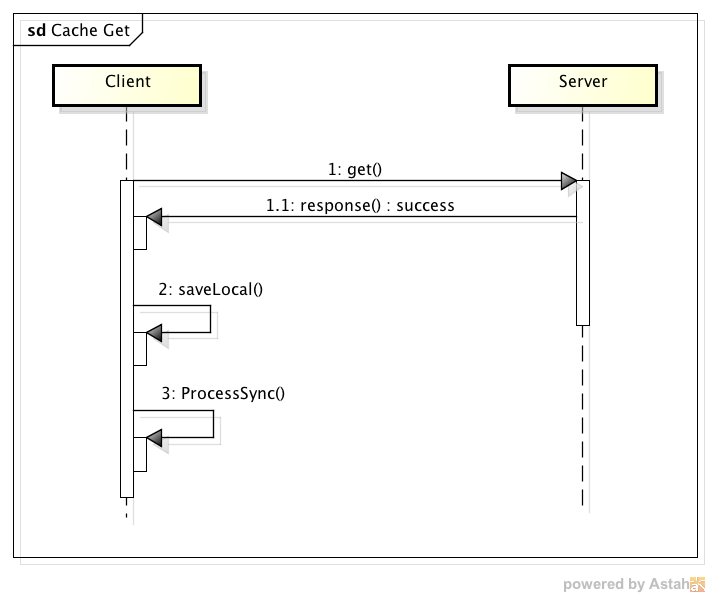
\includegraphics[width=0.8\linewidth]{content/images/Cache-Get}
\caption{Abrufen vom Server}
\label{pic:cacheGet}
\end{figure}
Die Synchronisation soll demnach im Anschluss einer Serververbindung geschehen, da man in diesem Fall sicher sein kann, dass eine Verbindung besteht, die dafür verwendet werden kann. Dementsprechend funktioniert auch der \textit{Post} oder das Hochladen von Daten (siehe Anhang \ref{sec:cachePost}).
	\chapter{Architektur}
\label{cha:architektur}
In diesem Kapitel werden die architektonischen Randbedingungen für die Entwicklung der Applikation beschrieben. Hierzu zählt, welche Anwendungsfälle in die späteren Prototypen und im schlussendlichen Messeprototyp gegeben sein muss. Daraus resultiert der Aufbau der Datenbank und die schlussendliche Systemarchitektur. Als Grundlage dient das Pflichtenheft. Dieses liegt dieser Arbeit gesondert im Anhang bei (siehe Anhang \ref{sec:Pflichtenheft}).

\section{Anwendungsfälle}
\label{sec:anwendungsfaelle}
Das Pflichtenheft sieht eine Unterteilung des Projekts in zwei aufeinanderfolgende Meilensteine vor (siehe Kapitel \ref{sec:meilenstein-plan}). Hierbei werden erst Proof-of-Concept-Prototyp entwickelt. Anschließend wird ein Prototyp zum Messeprototyp weiterentwickelt. \\
Für diese beiden Prototypen müssen andere bzw. erweiterte Anwendungsfälle implementiert werden. Darum werden nachfolgend für die beiden Implementierungsschritte die Anwendungsfälle einzeln aufgeschlüsselt. 
\subsection{Anwendungsfälle für Meilenstein 1 (Proof-of-Concept-Phase)}
\label{ssec:anwendungsfaelle-poc}
Aus dem Pflichtenheft ergeben sich folgende Anwendungsfälle für die erste Phase des Projekts:
\begin{itemize}
\item Es soll möglich sein, sich an der Anwendung anzumelden
\item Es soll möglich sein, eine Entität mit Daten (Trainingsplan, Training oder Übung), unabhängig von der Verbindung zum Web Service, persistent anzulegen, zu ändern und zu speichern
\item Optional soll sich ein Nutzer an der Anwendung registrieren können
\end{itemize}

\begin{figure}[h]
\centering
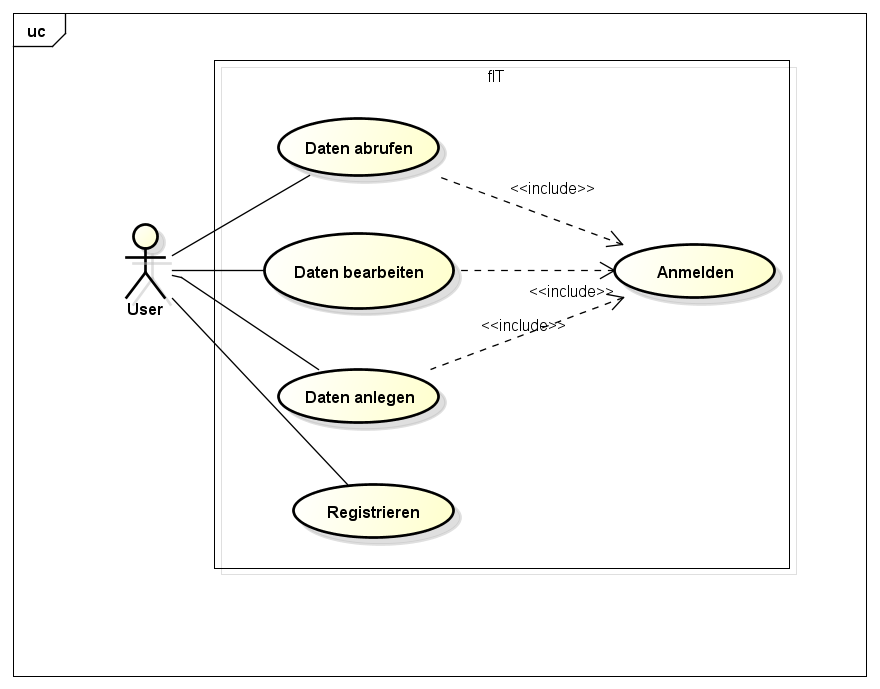
\includegraphics[width=0.8\linewidth]{content/images/UseCase-Proof-of-Concept.png}
\caption{Use-Cases Proof-of-Concept}
\label{pic:usecase-poc}
\end{figure}

\subsection{Anwendungsfälle für Meilenstein 2 (Messeprototyp-Phase)}
\label{ssec:anwendungsfaelle-messe}
Für den Meilenstein 2 werden die bereits vorgestellten Anwendungsfälle weiter verfeinert. Daraus ergeben sich folgende Anwendungsfälle:
\begin{itemize}
\item Ein Nutzer soll sich an der Anwendung anmelden können.
\item Ein Nutzer soll seine eigenen Trainingsplan-Daten abrufen können
\item Ein Nutzer soll zu einem seiner Trainingspläne alle zugehörigen Übungen abrufen können
\item Ein Nutzer soll zu einer dieser Übungen seine bisherigen Trainingsdaten abrufen können
\item Ein Nutzer soll zu einer Übung ein neues Training anlegen können
\item Alle nicht-optionalen Anwendungsfälle müssen unabhängig von einer Serververbindung funktionieren und eventuell anfallende Daten dauerhaft speichern.
\item Optional: Ein Nutzer soll eine Statistik der letzten Trainings zu einer Übung abrufen können. Neu erstellte Trainingsdaten aktualisieren diese Statistik
\item Optional: Ein Nutzer soll sich an der Applikation registrieren können
\item Optional: Ein Nutzer mit der Rolle \textit{Administrator} soll neue Übungen anlegen können
\end{itemize}

\begin{figure}[h]
\centering
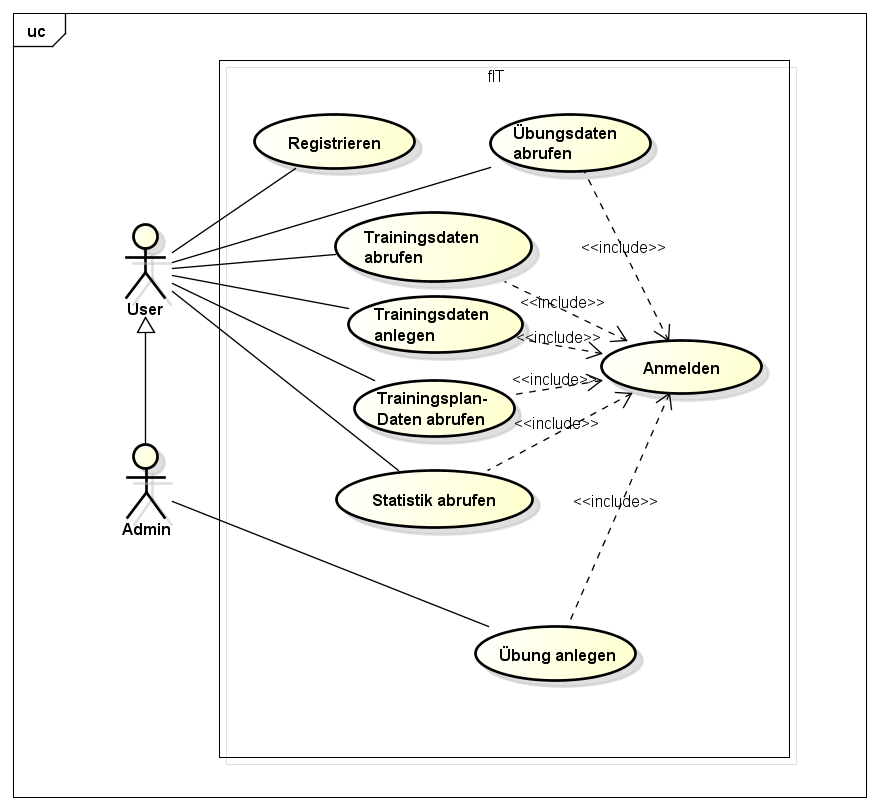
\includegraphics[width=0.8\linewidth]{content/images/UseCase-Messeprototyp.png}
\caption{Use-Cases Messeprototyp}
\label{pic:usecase-messe}
\end{figure}
\newpage
\section{Datenbank-Entwurf}
\label{sec:Datenbank-Entwurf}
Aus den definierten Anwendungsfälle ergibt sich die Struktur für die Datenbank. Als Grundlage werden die Anwendungsfälle des zweiten Meilensteins genutzt, um spätere Anpassungen nach Beendigung des ersten Meilensteins zu vermeiden.

\begin{figure}[h]
\centering
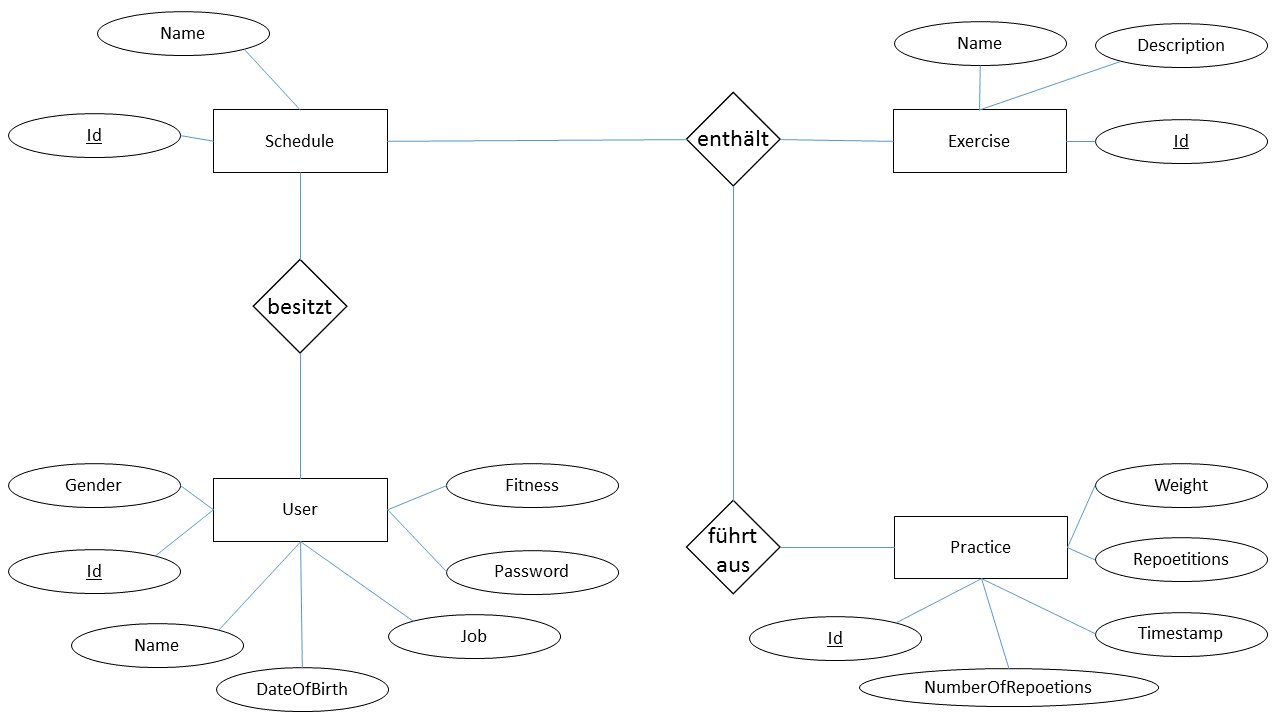
\includegraphics[width=0.8\linewidth]{content/images/DB-Entwurf.png}
\caption{Datenbank-Entwurf}
\label{pic:db-entwurf}
\end{figure}

\section{Programmarchitektur}
\label{sec:programmarchitektur}
Da verschiedene Clients implementiert werden sollen, ist es sinnvoll das Projekt als Mehrschichtenarchitektur für verteilte Anwendung zu implementieren. \\
Der Server hält dabei die Funktionen zur Nutzung durch die Clients vor. Konkret greift der Server per \gls{OR-Mapper} auf die Datenbank zu, bereitet die Daten in der Applikationsschicht auf und reicht sie über eine \ac{REST}-Schnittstelle an die anfragenden Client weiter. Eine detaillierte Beschreibung zu \ac{REST} wird in Kapitel \ref{sec:definition-rest} gegeben. Bei dieser Kommunikation muss gewährleistet sein, dass ein Nutzer nur die Daten abrufen darf, für die er autorisiert wurde. \\
Clientseitig werden Daten in einer Caching-Schicht zum Schutz vor eventuellen Verbindungsabbrüchen zwischengespeichert. Anschließend werden die erhaltenen Daten auf dem Endgerät für die Anzeige aufbereitet und angezeigt. \\
Abbildung \ref{pic:architecture} bildet diesen Aufbau grafisch ab:
\begin{figure}[h]
\centering
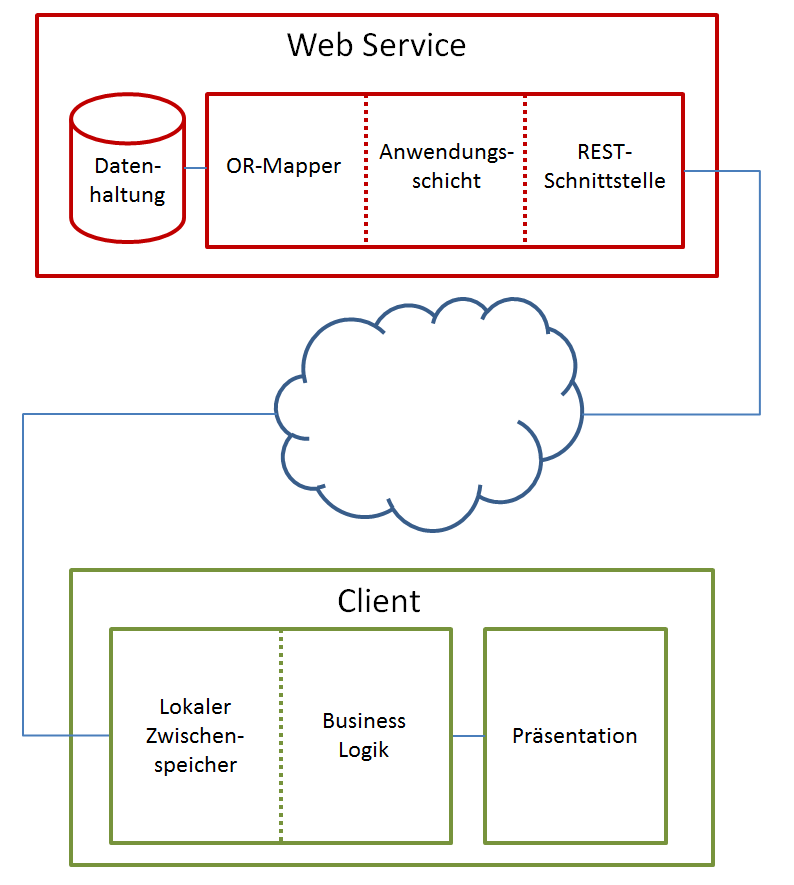
\includegraphics[width=0.7\linewidth]{content/images/Aufbau-Architektur.png}
\caption{Aufbau der Anwendung}
\label{pic:architecture}
\end{figure}

\newpage
\section{Rollen-Konzept}
\label{sec:rollen-konzept}
Im Pflichtenheft wird für den zweiten Meilenstein eine Unterscheidung in den Berechtigungen gemacht. So dürfen beispielsweise nur Administrationen neue Übungen anlegen. Darum ist es nötig, ein Rollenkonzept zu entwickeln, der den Zugriff auf bestimmte Ressourcen reguliert. \\
Aus den Aussagen, die im Pflichtenheft getroffen wurden, geht hervor, das sich der Nutzer in einer der nachfolgenden Status befindet, wenn er auf den Web Service zugreifen will: 
\begin{itemize}
\item unautorisiert \\
Der Nutzer hat sich noch nicht gegenüber des Web Server authentifiziert. In diesem Status kann der Nutzer sich mit seinen Anmeldedaten einloggen oder als neuer Nutzer an der Web Applikation registrieren.
\item Rolle \textbf{Nutzer}\\
Jeder angemeldete Nutzer besitzt die Rolle \textit{Nutzer}. Ein normaler Nutzer kann seine Daten einsehen. Dies beinhaltet seine Trainingspläne, deren Übungen und die dazu angelegten Trainingseinheiten.
\item Rolle \textbf{Administrator}\\
Ein \textit{Administrator} ist ebenfalls ein Nutzer. Er kann zusätzlich neue Übungen anlegen. 
\end{itemize}
	\chapter{Aspekte der Realisierung}
\label{cha:realisierung}
In diesem Kapitel werden allgemeine Komponenten für die Umsetzung dieses Projektes beschrieben. Dabei werden jeweils nur diese Techniken vorgestellt, welche von mehreren Komponenten genutzt werden, sodass sie in den jeweils dafür vorgesehenen Kapiteln mehrfach genannt werden müssten. \\
Als generelle Aussage ist zu erwähnen, dass versucht wurde, möglichst viele Entwicklungswerkzeuge eines Unternehmens zu benutzen um mögliche positive Synergieeffekte in Form von leichter Kommunikation zwischen den gewählten Komponenten zu gewährleisten. Zur Umsetzung dieses Projekts wurden weitestgehend die Produkte der Softwarefirma \textit{Microsoft} genutzt.

\section{Entwicklungsumgebung}
\label{sec:entwicklungsumgebung}
Für die Entwicklung sämtlicher Komponenten wurde \textit{Microsoft Visual Studio 2015 Community Edition} (kurz \textit{Visual Studio}) benutzt. Hierbei handelt es sich um die Standard-Entwicklungsplattform von \textit{Microsoft}. Diese Entscheidung wurde aus Gründen getroffen:
\begin{itemize}
\item Die Clients sollen durch die Drittanbieter-Frameworks \textit{Xamarin} und \textit{AngularJs} umgesetzt werden. Beide Frameworks sind entweder bereits in die Entwicklungsumgebung integriert oder können leicht nachträglich zum Projekt hinzugefügt werden. Die hierfür benutzten Programmiersprachen \textit{C\#} und \textit{Javascript} bzw. den kompletten \ac{Web Stack} werden vollständig mit gängigen \ac{IDE}-Features wie Autovervollständigung, Syntax-Highlighting und Debugger unterstützt. 
\item Die Entwicklung von Web Anwendungen wird erheblich erleichtert, da \textit{Visual Studio} mit einem integrierter Webserver ausgeliefert wird. Dadurch können entwickelte Applikationen direkt lokal getestet werden, ohne, dass ein zusätzlicher Webserver installiert oder die Anwendung auf einen Webserver deployt werden muss.
\item Eine starke Integration von anderen \textit{Microsoft} Produkten. Hierzu zählen die Hosting-Plattform \textit{Microsoft Azure} und das Datenbank-System \textit{Microsoft SQL Server}.
\item Die Entwicklungsumgebung kann benötigte Komponenten und deren Abhängigkeiten durch den integrierten Paketmanager nachladen. Dadurch entfällt das nachträglichen Herunterladen von DLLs, wodurch Kompatibilitätsprobleme verringert werden.\footcite{online:VisualStudio}
\end{itemize}
\section{Datenbank-System}
\label{sec:DB-System}
Als Datenbanksystem wurde ebenfalls die Lösung von \textit{Microsoft} verwendet. Hierbei handelt es sich um \textit{Microsoft SQL Server}. Durch die einheitliche Nutzung von Microsoft-Produkten kann für den Zugriff auf die Datenbank der \ac{OR-Mapper} genutzt werden. Dieser erlaubt es, direkt aus Modell-Klassen Datenbank-Entitäten zu entwickeln. Dieser Vorgang wird in Kapitel \ref{ssec:aufbau-server-db} näher erläutert\footcite{online:SQLServer}.
\section{Hosting-Plattform}
\label{sec:Hosting-Plattform}
Sowohl der Web Service als auch die Web-Application-Client müssen im Internet verfügbar gemacht werden, damit so von überall erreichbar sind. Hierzu biette \textit{Microsoft} die Hosting-Plattform \textit{Azure} an. Diese ermöglicht es, direkt aus \textit{Visual Studio} heraus seine Webanwendung zu veröffentlichen. Gleichzeitig lässt sich eine Datenbank hosten, welchen der Webservice direkt benutzen kann. Zusätzlich ist Azure sehr gut skalierbar, was den Einsatz als Hosting-Plattform für kleine Prototyp-Projekte optimal unterstützt\footcite{online:Azure}.
\section{Versionsverwaltung}
\label{sec:versionsverwaltung}

\section{Dokumentationslösung}
\label{sec:dokumentationslösung}

 	
	\chapter{Realisierung der serverseitigen Implementierung}
\label{cha:server-impl}
In diesem Kapitel wird näher auf die Implementierung des in Kapitel \ref{cha:architektur} besprochenen Webservices eingegangen. Es enthält eine Übersicht über die genutzten Komponenten und die konkreten Techniken, welche für die Implementierung genutzt wurden. Anschließend werden nochmal besonders auf Sicherheitsaspekte in Verbindung mit RESTful-Architekturen eingegangen. 

\section{Was ist ein Webservice?}
\label{sec:definition-webservice}
Um verteilte Systeme aufzubauen ist es nötig, eine Struktur zu implementieren, mit der Maschinen untereinander kommunizieren können. Diese Aufgabe übernehmen Webservices. Sie stellen innerhalb eines Netzwerkes Schnittstellen bereit, damit Maschinen plattformübergreifend Daten austauschen können. Hierbei wird meistens HTTP als Träger-Protokoll genutzt um eine einfache Interoperabilität zu gewährleisten.\footcite{Definition-Webservice}Die angeforderten Daten werden in der Regel im XML- oder JSON-Format übermittelt. 

\subsection{RESTful Webservices}
\label{sec:definition-rest}
Da Webservices in der Regel \ac{HTTP} als Protokol verwenden, wurde die Idee zur Implementierung eines Webservices erweitert, um die Möglichkeiten des Protokolls vollständig zu benutzen. Mit einem Rest-Server bzw. einem RESTful Webservice bezeichnet man einen Webservices, welcher die strikte Nutzung von HTTP als Programmierparadigma umsetzt. REST bedeutet \textit{Representational State Transfer}. Dies meint, dass sich, wie im Internet üblich, hinter einer \ac{URI}, genau eine einzige Resource verbirgt. Bei einer Resource geht man von Daten aus. Im Gegensatz zu anderen Webservice-Implementierungen stellen Restful Webserver keine Methoden oder aufrufbare Funktionalitäten zu Verfügung. Diese Daten werden vom Rest-Server über eine eindeutige URL bereitgestellt. Dies hat den Vorteil, dass die Schnittstele leicht und eindeutig beschrieben werden kann, da ein Aufruf einer URL an den Rest-Server immer die gleichen Daten liefert. 

In den meisten Fällen, wie auch in den Anwendungsfällen dieser Arbeit, soll der Webservice \ac{CRUD}-Funtionalitäten

Da das statuslose Protokoll HTTP zum Datenaustausch genutzt wird, muss ein Restful Webservice so implementiert werden, dass alle Informationen, welche für die Kommunikation benötigt werden, bei jeder Kommunikation mitgesendet werden. Was vordergründig als Nachteil erscheint ist ein wesentlicher Vorteil. Dadurch, dass jeder Request alle nötigen Informationen mitliefert, ist es nicht nötig, Sitzungen auf dem Server zu verwalten. Dadurch kann ein Restful Webservice sehr leicht skaliert werden. 

% Abschnitt über unterschiedliche Repräsentationen


\section{Aufbau der Komponenten}
\label{sec:aufbau-Komponenten}

\subsection{Aufbau der Datenbank}
\label{ssec:aufbau-server-db}

\subsection{Aufbau der WebApi}
\label{ssec:aufbau-webapi}

\subsubsection*{Swagger}
\label{sssec:Swagger}

\section{Authentifizierung \& Autorisierung}
\label{sec:server-authorisierung}

\subsection{OAuth2}
\label{ssec:oauth2}

\subsection{JWT and Bearer Token}
\label{ssec:jwt-bearer}

\subsection{Zugriff per CORS}
\label{ssec:cors}
	\chapter{Realisierung der clientseitigen Implementierung als native App}
\label{cha:native-app}
Dieses Kapitel widmet sich der Implementierung der nativen Applikation. Im Kapitel \ref{cha:architektur} wurde eine grobe Übersicht zu der Umsetzung und der Funktionsweise dieser \ac{App} gegeben, die nun verfeinert wird.
Dabei werden folgend die verwendeten Komponenten und Techniken erläutert und die Zusammenhänge zwischen den Techniken dargestellt.
\section{Allgemeine Funktionsweise einer Android-App}
\label{sec:definition-android}
Grundlegend für die Entwicklung einer Android-App ist das Wissen über die Basis des Systems, auf dem entwickelt wird. 
Bei dem Betriebssystem \ac{Android} handelt es sich um eine Art eines \ac{monolithisch}en Multiuser-\ac{Linux}-Systems. \footcite{Android-Fundamentals}
Dieses Betriebssystem stellt die Hardwaretreiber zur Verfügung und führt die Prozessorganisation, sowie die Benutzer- und Speicherverwaltung durch.\footcite[S. 19ff.]{Android-BeckerPant}
Jede Applikation wird in einem eigenen Prozess gestartet. In diesem Prozess befindet sich eine \ac{Sandbox}, die eine virtuelle Maschine mit der Applikation ausführt. Die Kommunikation aus der Sandbox heraus kann nur über Schnittstellen des Betriebssystems geschehen. Diese Einschränkung sorgt für Sicherheit im System, da ein Prinzip der minimalen Rechte eingehalten wird. Demnach kann eine Applikation nur auf zugewiesene und freigegebene Ressourcen im System zugreifen. Ein weiterer Vorteil dieser internen Architektur liegt in der Robustheit des Systems. Wenn eine Applikation durch Fehler terminiert, wird nur der allokierte Prozess beendet und das Betriebssystem bleibt von diesem Problem unberührt. \footcite{Android-SystemPermissions}
Android-Applikationen werden in der Programmiersprache \ac{Java} geschrieben, mit einem Java-\ac{Compiler} kompiliert und dann von einem Cross-Assembler für die entsprechende \ac{VM} aufbereitet. Das Produkt ist ein ausführbares \ac{.apk}-Paket.\footcite{Android-Fundamentals}
Im Folgenden werden die Android-Komponenten, die für die Umsetzung relevant sind, genauer betrachtet.
\subsection{User Interfaces}
\label{ssec:android-ui}
\textit{User Interfaces} sind die Bildschirmseiten der Android-Applikation. Über diese Seiten wird die Benutzerinteraktion geführt. Das \textit{User Interface} besteht aus zwei Arten von Elementen. Zum einen aus \textit{Views}, die es ermöglichen direkte Interaktionen mit dem Benutzer zu führen. Zu nennen sind dabei \textit{Buttons}, Textfelder und Checkboxen. Als zweites werden \textit{View Groups} verwendet, um \textit{Views} sowie andere \textit{View Groups} anzuordnen.\footcite[S. 40f.]{Android-BeckerPant}\\
Das \textit{User Interface Layout} ist durch eine hierarchische Struktur gekennzeichnet. Zum Anlegen einer solchen Struktur gibt es verschiedene Möglichkeiten. Zum einen kann man ein \textit{View}-Objekt anlegen und darauf die Elemente platzieren. Aus Gründen der Performance und der Übersicht ist die Möglichkeit einer \ac{XML}-Datei jedoch zielführender. Aus den Knoten der erstellten Datei werden zur Laufzeit \textit{View}-Objekte erzeugt und angezeigt. Die erzeugten \textit{UIs} werden unter \textit{res/layout} im Android-Betriebssystem hinterlegt. Des Weiteren können Ressourcen in den \textit{UIs} verwendet werden. Unter Ressourcen versteht man Elemente, die zum Verzieren von Oberflächen verwendet werden können. Darunter fallen bespielsweise Grafiken oder \textit{Style-Sheets}, die über den jeweiligen Ressourcen-Schlüssel aufgerufen und verwendet werden.\footcite{Android-UI}
\subsection{Activities}
\label{ssec:android-activities}
\textit{Activities} gehören zu den App-Komponenten, da sie ein grundsätzlicher Bestandteil einer Applikation sind. Es gibt im Normalfall mehrere \textit{Activities} in einer App.\\
Die eigentlichen Aufgaben liegen in der Bereitstellung eines Fensters, das dann auf den \textit{Screen}, der für die App vom Betriebssystem bereitgestellt wird, gelegt wird. Das Fenster ist im Anschluss für die Annahme von Benutzerinteraktionen bereit.\footcite[S. 40]{Android-BeckerPant} Das Fenster wird mit Hilfe des Aufrufs \textit{SetContentView()} aufgerufen. Zur Benutzerinteraktion werden dann die bereits vorgestellten \textit{View}-Elemente verwendet. Die \textit{Activity} ist folgend für die Verarbeitung und Auswertung der Eingaben verantwortlich.\\
In jeder Applikation muss es eine \textit{MainActivity} geben, die beim Start der Applikation vom Android-Betriebssystem gestartet wird. Zudem muss eine \textit{Activity} im AndroidManifest mit dem Attribut \textit{Launcher} versehen werden, um diese dann als Einstiegspunkt in das Menü des Betriebssystems zu setzen. Dabei ist empfehlenswert, dass dieselbe \textit{Activity} sowohl das Main- als auch Launcher-Attribut erhält.\\
Das Manifest liegt im Root-Ordner der App und stellt dem Betriebssystem wichtige Informationen der Applikation zur Verfügung. Dieses Manifest wird vor Ausführung der App analysiert und ausgewertet. Darin kann beispielsweise festgelegt werden, welche Komponenten oder anderen Applikationen auf entsprechende \textit{Activities} zugreifen dürfen. Wenn eine \textit{Activity} nicht von außerhalb der App erreichbar sein soll, sollte kein Intent-Filter gesetzt werden.\\
Da eine App normalerweise aus mehreren \textit{Activities} besteht, müssen diese gestartet werden und untereinander kommunizieren. \textit{Activities} starten sich gegenseitig, weshalb der Aufruf einer \textit{Activity} aus einer anderen erfolgt. Um eine neue \textit{Activity} starten zu können, ist ein \textit{Intent} von Nöten.\footcite[S. 135ff.]{Android-BeckerPant}
Ein \textit{Intent} ist ein Nachrichtenobjekt innerhalb von Android, welches zur Kommunikation zwischen App-Komponenten verwendet wird. In diesem Fall zwischen zwei \textit{Activities}. Zur Erstellung benötigt es den Namen der zu startenden Komponente, um eine Verbindung dorthin aufbauen zu können, und eine \textit{Action}, die ausgeführt werden soll. Zudem können Daten übergeben werden, die anschließend als Datenpakete mit dem Aufruf der Komponente mitgegeben werden. Diese Daten sind dann in der gestarteten Komponente aus dem dort vorhandenen Intent auslesbar. Zusätzlich gibt es die Möglichkeit Aktionen vom Betriebssystem ausführen zu lassen. Beispielsweise kann man einen \textit{Intent} mit der Aktion zum Starten des Email-Programms übergeben und die entsprechend im Betriebssystem hinterlegte Applikation zum Schreiben von Emails wird geöffnet.\footcite{Android-Intent}\\
%ActivityLifecycle-Bild
\begin{figure}[!htbp]
\centering
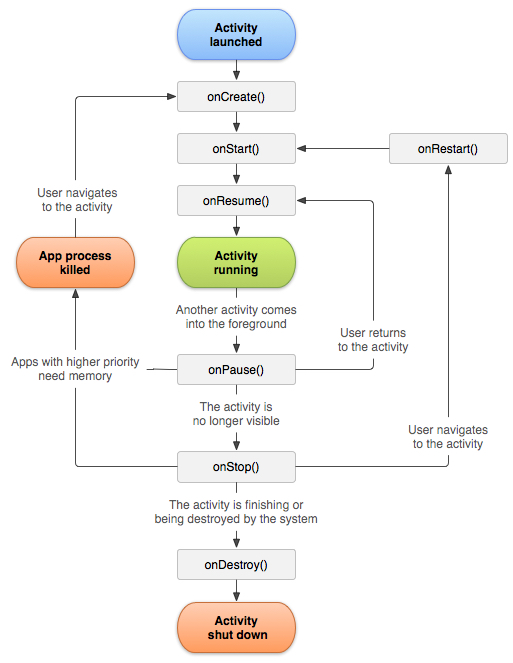
\includegraphics[width=0.8\linewidth]{content/images/Android-ActivityLifecycle}
\caption{Android Activity-Lifecycle}
Quelle: https://developer.android.com/guide/components/activities.html
\label{pic:androidActivityLifecycle}
\end{figure}
Eine \textit{Activity} kann drei Stati in einem \textit{Lifecycle} einnehmen. Zum einen kann die \textit{Activity} im Status \textit{Resumed} - oft auch \textit{Running} genannt - sein und damit momentan im User-Fokus stehen, also im Vordergrund der App sein und die Interaktionen entgegennehmen. Des Weiteren kann eine \textit{Activity} pausieren, wenn eine andere im User-Fokus steht. Dabei ist der \textit{View} der betrachteten \textit{Activity} jedoch immer noch teilweise sichtbar, da der darüberliegende \textit{View} zu Beispiel nicht den gesamten Bildschirm in Anspruch nimmt. Anders verhält es sich, wenn der \textit{View} der betrachteten \textit{Activity} komplett überdeckt ist. Dann befindet sich die \textit{Activity} nämlich im Status \textit{Stopped}. Die Abbildung \ref{pic:androidActivityLifecycle} zeigt die möglichen Übergänge zwischen den verschiedenen Stati.\footcite{Android-Activities}\\
Essentiell ist die \textit{OnCreate}-Methode, in der Initialisierungen durchgeführten werden sollten und der View gestartet wird. Kehrt der Benutzer nach einer Bearbeitungspause zu der aktuellen \textit{Activity} zurück, wird \textit{OnResume} ausgeführt.\\
Die \textit{OnStop}-Methode sollte zur Persistierung von Daten verwendet werden und die darauf folgende Methode \textit{OnDestroy} alle Aufrufe eines Destruktors enthalten.\footcite[S. 289]{Android-BeckerPant}\\
Die Methoden sollten aus Performancegründen jedoch minimal und agil gehalten werden.
\subsection{Services}
\label{ssec:android-services}
\textit{Services} sind, genauso wie \textit{Activities}, App-Komponenten, die zu den Grundbausteinen einer Android-App gehören. \textit{Services} unterscheiden sich jedoch hinsichtlich ihrer Aufgaben stark von \textit{Activities}. So sind sie dazu da, Aufgaben im Hintergrund zu erledigen. Zudem besitzen sie keinen zugehörigen \textit{View}, sondern werden von anderen App-Komponenten, wie beispielsweise einer \textit{Activity} gestartet.\footcite[S. 163]{Android-BeckerPant} Sie laufen im \textit{Main-Thread} des Prozesses der aufrufenden Komponente. Ein \textit{Service} erstellt weder einen eigenen \textit{Thread}, noch einen eigenen Prozess zur Abarbeitung der Aufgaben.\footcite{Android-Services} Diese Eigenschaft der \textit{Services} muss vom Entwickler bedacht werden. Denn daraus kann man ableiten, dass rechenintensive Aufgaben in einem explizit gestarteten \textit{Thread} abgearbeitet werden sollten, um Fehler der Art \ac{ANR} zu vermeiden und die Benutzeroberfläche nicht unnötig zu verlangsamen. Ein Vorteil besteht jedoch darin, dass \textit{Services} Aufgaben auch dann noch ausführen können, wenn die App, zu der sie gehören, geschlossen wurde. So können noch nicht abgeschlossene \textit{Up-} oder \textit{Downloads} noch beendet werden oder das Abspielen von Musik bei ausgeschaltetem Bildschirm fortgeführt werden.\footcite[S. 161f.]{Android-BeckerPant}\\
Bei Android wird grundsätzlich zwischen zwei Arten von \textit{Services} unterschieden. Zum einen gibt es \textit{Started-Services}, die durch eine App-Komponente mit dem Befehl \textit{StartService()} gestartet werden. Grundsätzlich ist dieser Aufruf uneingeschränkt von allen App-Komponenten möglich, soweit die Einstellungen im Android-Manifest diese zulassen. Weiterhin laufen \textit{Started-Services} im Hintergrund der App weiter, auch wenn die Komponente, die den \textit{Service} gestartet hat, zerstört oder beendet wurde. Deshalb führt diese Art des \textit{Services} im Normalfall eine Aufgabe aus und stoppt sich anschließend nach der Fertigstellung selbst. Auf der anderen Seite gibt es \textit{Bound-Services}, die durch einen Aufruf von \textit{BindServcice()} einer anderen App-Komponente gestartet werden. In diesem Schritt verbinden sich die Komponente und der \textit{Service} über eine Art \textit{Client-Server Interface}, das zur Kommunikation bereitgestellt wird. Dieses \textit{Interface} ist vom Typ \textit{IBind} und sorgt für den Austausch von \textit{Requests} und \textit{Results}. Die größte Besonderheit eines \textit{Bound-Services} besteht darin, dass der \textit{Service} nur so lange besteht, wie mindestens eine Komponente an diesen gebunden ist. Natürlich ist es möglich, dass sich mehrere Komponenten gleichzeitig an diesen \textit{Service} binden können. Löst sich jedoch die letzte Komponente wieder, wird der \textit{Service} zerstört. Es gibt auch Mischformen dieser beiden \textit{Service}-Arten, die abhängig von der zu leistenden Aufgabe gewählt werden können.\footcite{Android-Services} 

%ServiceLifecycle-Bild
\begin{figure}[!h]
\centering
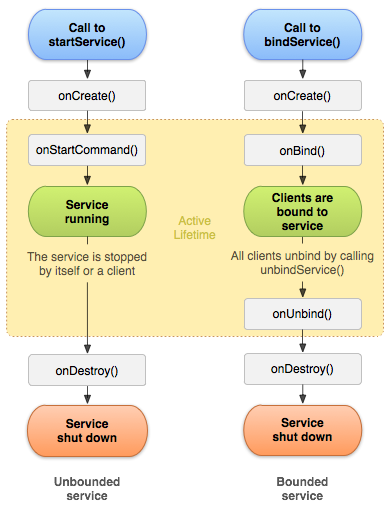
\includegraphics[width=0.5\linewidth]{content/images/Android-ServiceLifecycle}
\caption{Android Service-Lifecycle}
Quelle: https://developer.android.com/guide/components/services.html
\label{pic:androidServiceLifecycle}
\end{figure}

Zum Erstellen eines \textit{Services} muss von der Klasse \textit{Service}, oder davon abgeleitete Klassen, geerbt werden. Danach müssen die vorgegebenen Methoden überschrieben werden, denn \textit{Services} besitzen, genauso wie \textit{Activities}, einen Lebenszyklus. Dabei muss jedoch wieder zwischen den beiden Arten von \textit{Services} unterschieden werden.\footcite[S. 168f.]{Android-BeckerPant}\\
Die Umrahmenden Methoden sollten, ähnlich zu den Methoden der \textit{Activities}, für die Initialisierung und Freigabe der verwendeten Komponenten sorgen. \textit{OnStartCommand()} wird immer dann aufgerufen, wenn der \textit{Service} wieder von einer Komponente aufgerufen wird. Dann befindet er sich im Zustand \textit{Running} und führt die ihm zugewiesenen Aufgaben durch. Wenn der \textit{Service} zerstört wird, sei es durch Speichermangel des \textit{Devices}, das Beenden durch eine Komponente oder den \textit{Service} selbst, wird \textit{OnDestroy()} ausgeführt.\\
\textit{Bound-Services} verhalten sich sehr ähnlich zu den \textit{Started-Services}, sind jedoch von dem Binden und Lösen von Komponenten abhängig und führen demnach die entsprechenden Methoden zur Ausführung ihrer Aktionen aus.\footcite{Android-Services}
\subsection{Prozesse und Threads}
\label{ssec:android-prozesse-threads}
Sobald eine Applikation gestartet wird, und keine Komponenten daraus bereits laufen, wird vom Android-Betriebssystem ein neuer Prozess mit einem dazugehörigen \textit{Main-Thread} erzeugt. Standardmäßig werden alle Operationen dieser App in diesem Prozess und diesem \textit{Thread} ausgeführt. Laufen Teile einer Applikation jedoch noch im Hintergrund, wie es bei Services möglich ist (siehe \ref{ssec:android-services}), und die App wird vom Benutzer erneut gestartet, so wird diese Komponente in dem noch bestehenden Prozess und \textit{Thread} eingepflegt.\\
Es gibt jedoch auch die Möglichkeit verschiedene App-Komponenten auf mehrere Prozesse zu verteilen. Dazu genügt ein Eintrag im Android-Manifest. Dadurch ist es dann auch möglich Komponenten verschiedener Applikationen in einem Prozess laufen zu lassen. Voraussetzung dafür ist, dass diese beiden Applikationen mit demselben Zertifikat generiert wurden und dieselbe Linux \textit{\ac{user ID}} besitzen.\footcite{Android-ProcessesThreads}\\
Prozesse können aber auch durch das Betriebssystem zerstört werden, wenn die Geräte-Ressourcen sich zum Beispiel dem Ende neigen und neue freigegeben werden müssen. Hierzu gliedert Android die Prozesse in eine Hierarchie ein und beendet die Prozesse, die zum Beispiel vom Benutzer seit längerer Zeit nicht mehr verwendet wurden oder keinen direkten Kontakt zur aktuellen Anzeige besitzen.\\
Der angesprochene \textit{Main-} oder auch \textit{\ac{UI-Thread}} beim Starten einer App, ist der Hauptakteur für die Kommunikation mit dem Betriebssystem. So werden alle Aufrufe an die Komponenten des \textit{Android UI toolkits} über diesen \textit{Thread} abgewickelt. Demnach müssen über diesen \textit{Thread} alle \textit{Callback}-Methoden von Systemeigenschaften, wie \textit{OnClick()}, darin bearbeitet werden. Daraus ergibt sich, dass aufwendige Aufgaben, die zum Beispiel Netzwerkverbindungen verwenden, in andere \textit{Threads} verlagert werden sollten, um dem Benutzer eine Oberfläche ohne lästige Wartezeiten zu ermöglichen. Einzige Einschränkung dabei ist, dass niemals von einem anderen \textit{Thread} als dem \textit{UI-Thread} auf \textit{\ac{Android UI toolkits}} zugegriffen werden darf. Diese Limitierung muss bei der Implementierung beachtet werden.\footcite[S. 160f.]{Android-BeckerPant}\\
Zum Umgehen dieser Problematik können asynchrone \textit{\ac{Tasks}} verwendet werden, die Aufgaben außerhalb des \textit{UI-Threads} ausführen. Auf das Ergebnis dieser Ausführungen kann dann wieder zugegriffen werden. Diese Umsetzung bietet einen leichteren Umgang mit \textit{Multithreading} für den Entwickler und genießt deshalb immer größere Beliebtheit.
\subsection{SQLite}
\label{ssec:android-sqlite}
SQLite ist eine in sich geschlossene und serverlose \ac{SQL}-Datenbank. Sie besteht aus einer \textit{In-Process}-Bibliothek, die es ermöglicht eine Datenbank ohne eigenen Server-Prozess zu betreiben. Dabei liegt die Datenbank mitsamt aller Tabellen, \textit{Views} und \textit{\ac{Trigger}} in einer einzigen Datei vor. Diese Datei ist zudem so konzipiert, dass sie plattformübergreifend zwischen 32- und 64-Bit-Systemen kopiert werden kann. Weitere Vorteile von SQLite liegen in der sehr sparsamen Speicherung der Daten und der, durch die gemeinfreie Lizenz, große Unterstützung durch Drittanbieter-Programmen. So gibt es für alle gängigen mobilen Systeme eine meist schon integrierte Unterstützung von SQLite-Datenbanken. Android unterstützt diese Datenbankart als präferierte Datenhaltung.\footcite[S. 226f.]{Android-BeckerPant}
\section{Was ist \textit{Xamarin Platform}?}
\label{sec:defintion-xamarin}
Xamarin Platform ist ein Produkt der Firma Xamarin, die ihren Sitz in San Francisco hat. Diese Firma entwickelt Software für die Erstellung von nativen Apps auf Basis des \textit{Open Source}-Projekts \ac{Mono}. Mono seinerseits hat mehrere Vorteile:
\begin{itemize}
\item \textbf{Popularität}\\Es kann auf die Erfahrung von Millionen C\# -Entwicklern zurückgegriffen werden.
\item \textbf{Höhere Programmiersprache} \\Es können die Vorteile von höheren Programmiersprachen verwendet werden. Zu nennen sind dabei besonders \textit{Threading}, automatische Speicherverwaltung und \textit{\ac{Reflection}}.
\item \textbf{Klassenbibliotheken}\\Die Verwendung von bestehenden Klassenbibliotheken erleichtern das Umsetzen komplexer Aufgaben.
\item \textbf{\textit{Cross-Platform}}\\Die fertiggestellte Software kann auf fast allen Systemen verwendet werden.
\end{itemize}
Damit können plattfomunabhängige Programme in C\# programmiert werden. Beliebtheit erlangte Mono mit dem Wunsch von Entwicklern Apps auf verschiedenen mobilen Betriebssystemen bereitstellen zu können und dabei Änderungen und die Entwicklung größtmöglich zu vereinen.\footcite{Xamarin-Multiplatform} Genau diese Wünsche werden mit \textit{Xamarin Platform} erfüllt. Vorher war es immer nötig drei Applikationen für die verbreitetsten mobilen Betriebssysteme zu entwickeln. Dies bedeutete, dass die \textit{Guidlines} der jeweiligen Systeme iOS, Android und Windows Phone analysiert und in den jeweiligen Programmiersprachen umgesetzt werden mussten.\footcite{Xamarin-Platform}
\subsection{Multiplattform-Unterstützung}
\label{ssec:xamarin-multiplattform}

%Xamarin-Platform-Bild
\begin{figure}[!h]
\centering
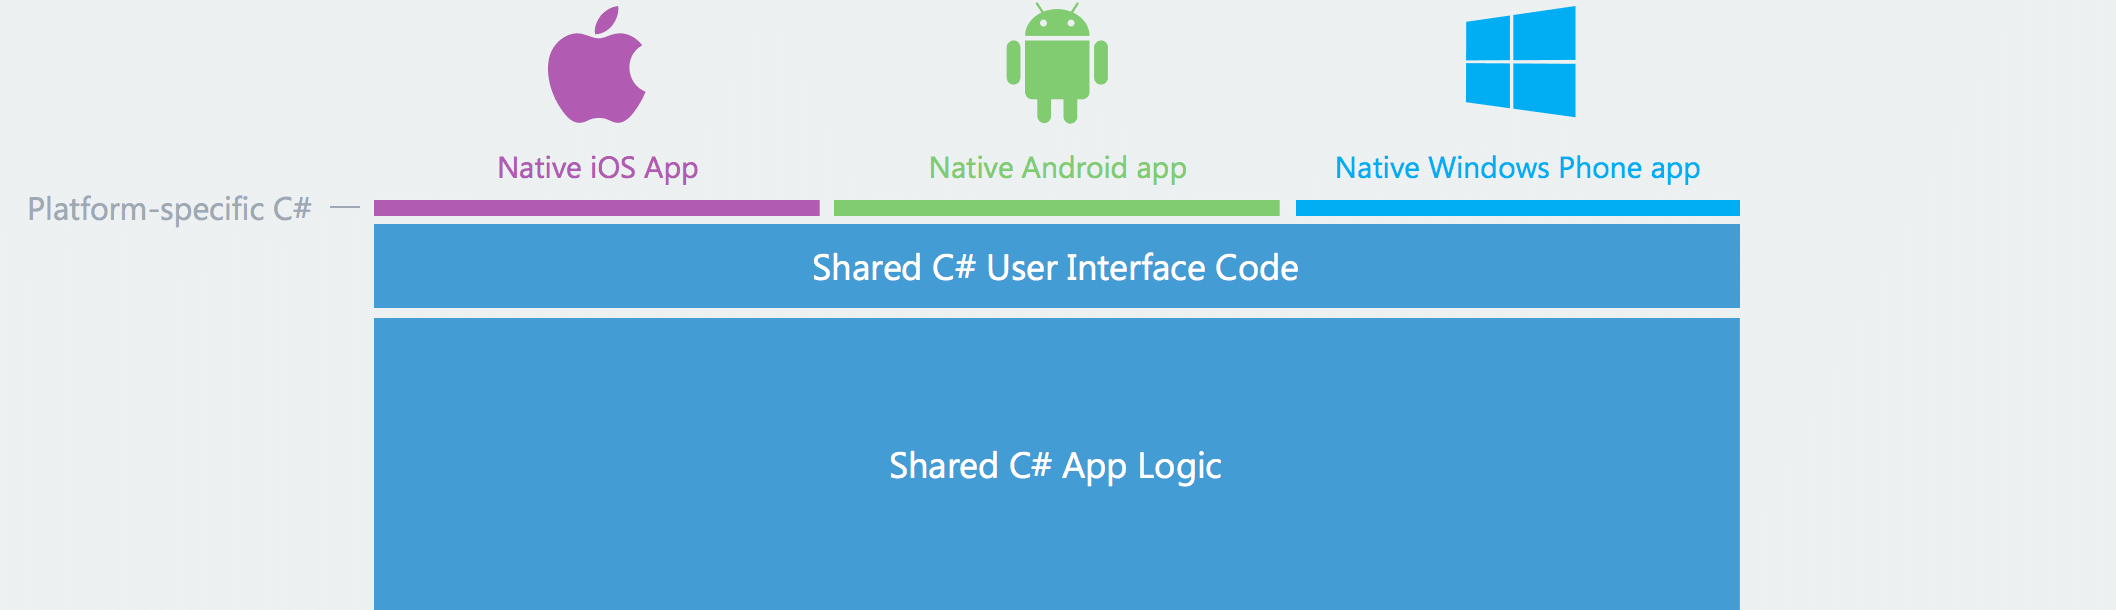
\includegraphics[width=\linewidth]{content/images/Xamarin-Platform}
\caption{Xamarin Platform}
Quelle: http://xamarin.com/platform
\label{pic:xamarinPlatform}
\end{figure}

Durch Xamarin Platform ist es möglich alle Funktionalitäten der gewünschten Betriebssysteme in vollem Umfang zu verwenden. Diese Tatsache liegt daran, dass erstellte Projekte in die nativen Sprachen des Systems überführt und dann normal kompiliert werden. Durch die Nutzung der Standard-Steuerelemente eines jeden Betriebssystems sorgt dafür, dass die Benutzer keinen Unterschied zu einer App erkennen können, die ausschließlich für ein Betriebssystem entwickelt wurde. Auch plattformspezifische Funktionen können verwendet werden. Zudem werden alle Vorteile der Programmiersprache C\# ausgenutzt.\footcite{Xamarin-Platform} So ist der Umgang mit asynchronen Funktionen in dieser Sprache zum heutigen Stand am besten gelöst. Des Weiteren können \textit{Shared Projects} zur Entwicklung verwendet werden, sowie \ac{PCL}s und \textit{\ac{NuGet}}-Pakete eingebunden werden, um den Funktionsumfang schnell und einfach erweitern zu können.\footcite{Xamarin-Multiplatform}
\subsection{Besonderheiten der Android-Umsetzung}
\label{ssec:xamarin-android}
Bei der Entwicklung einer Android-App mit Hilfe von Xamarin Platform vereint man die Vorteile zweier Systeme. Zum einen hat man den Vorteil der freien und starken Entwicklungsumgebung Visual Studio in Kombination mit C\#, zum anderen kann man alle Besonderheiten der Android-Entwicklung einbeziehen und verwenden.\\
So muss man am Anfang der Entwicklung auswählen, welche Android-\ac{API} als Minimalvoraussetzung verwendet werden soll und welche Version vorrangig unterstützt werden soll. Zweifellos ist es möglich die von dem \textit{Device} verwendete Android-Version abzufragen und dementsprechend die Funktionalität der App anzupassen.
Zudem können \textit{Java-Packages} eingebunden und verwendet werden, um bekannte Funktionen auch in C\# verwenden zu können.\\
Eine sehr große Unterstützung ist das automatische Führen des Android-Manifestes. Dabei werden zwar nur rudimentäre Einstellungen aus der Entwicklung übernommen, aber auch diese Unterstützung ist für Neulinge auf dem Gebiet der Android-Entwicklung eine gute Beihilfe.
\subsection{Android Emulator}
\label{ssec:xamarin-emulator}
Zum Testen der Android-App konnte ein Emulator verwendet werden, der in dem Xamarin-Plugin für Visual Studio bereitgestellt wurde. Damit konnten dann verschiedene Szenarien, wie Verbindungsverlust oder Speicherknappheit, nachgestellt werden. Für die App wurde das Android-API-Level 19 als Minimal-Anforderung gewählt. Das und \textit{Target}-Level wurde auf das API-Level 21 gesetzt. Dies steht für Android 5.0 mit dem Namen Lollipop. Damit sollte eine große Abdeckung von Android-Geräten bewerkstelligt werden.\footcite{Xamarin-API}
\section{Eigene Umsetzung}
\label{sec:nat-umsetzung}
Im folgenden wird auf die Umsetzung der nativen Android-Applikation mit Hilfe von Xamarin Platform eingegangen. Anfangs wurde beim Anlegen des Projektes das Android-API-Level, wie oben beschrieben, auf 19-21 gesetzt und die Entwicklung darauf abgestimmt.

\subsection{Anlegen der Layouts}
\label{ssec:nat-layouts}
Es müssen verschiedene Oberflächen angelegt werden. Darunter sind Login-Fenster, Übersichtsseiten, die die Trainingspläne und Übungen anzeigen, und eine Seite zum Eintragen von Trainingsdaten.\\
Beim Aufbau der Oberflächen sind die Schritte eindeutig identifizierbar, da diese Prozedur für alle \textit{Layouts} gleich abgehandelt werden sollte.\\
Zuerst wird ein \textit{Layout} angelegt und die Bedienelemente (\textit{Widgets}) darauf angeordnet. Dazu kann man \textit{ViewGroups} zur Gruppierung verwenden und die Ausrichtung auf dem Fenster wird mit Hilfe von \textit{Layouts} möglich.\footcite[Vgl. S. 58ff.]{Android-BeckerPant}\\
Probleme entstanden dabei jedoch nur manchmal bei der Ausrichtung von \textit{Widget}-Elementen, die aber zügig gelöst werden konnten.\\
Des Weiteren muss für die Oberfläche dann eine dazugehörige \textit{Activity} angelegt werden, die das Fenster aufruft und die Interaktionen hinter den \textit{Buttons} ausführt.\\
Zum Anzeigen der Login- und Registrieren-Oberflächen wurden Dialoge verwendet, um dem Benutzer zu zeigen, dass sich die Interaktion zum Anmelden vor dem Zugang zu der eigentlichen Applikation vollzogen werden muss.\\
Auf der Seite zur Registrierung sollen Daten über den Fitnesszustand, das Geschlecht und die körperliche Betätigung aus einer Auswahl wählbar sein. Dazu sollten dementsprechend \textit{Spinner}, scrollbare Auswahlfelder, verwendet werden. Dabei lag die Schwierigkeit jedoch in der Belegung mit den auswählbaren Werten. Diese mussten zuerst eingesetzt und dann nach der Übergabe an die \textit{Activity} wieder zurückformatiert werden. Es werden von der Oberfläche nämlich nur \textit{Strings} übergeben. 
Zur Aufnahme der Daten Geschlecht, Job und Beruf gibt es vorher definierte Daten für die Eingabe auf dem Server. Dabei hat sich anfangs die Schwierigkeit ergeben, dass die \textit{Spinner}, die scrollbaren Auswahlfelder, mit den festgelegten Daten besetzt und dann in dem entsprechenden Datentypen wieder ausgelesen werden müssen. Die Belegung der \textit{Spinner} erfolgt über einen typisierten \textit{ArrayAdapter}, der die Werte des übergebenen \textit{Enums} ausgibt. Das Einlesen des ausgewählten Wertes wird über jeweils eine ausgelagerte Funktion geregelt, die die Auswahl, die als \textit{String} erhalten wird, in den jeweiligen Typ überführt. Anhand der erhaltenen \textit{ServerException} wird dann ausgegeben, welche Eingabe für die Registrierung falsch eingegeben wurde. Dies ist auch einer der Gründe, weshalb die Registrierung nur im Online-Modus der App unterstützt wird. Zudem muss der Server überprüfen, ob der Benutzername verwendet werden kann.\\
Nach erfolgreicher Registrierung verschwindet der Dialog wieder und die Konnektivitätsanzeige der Startseite wird mit dem aktuellen Status belegt. Dies geschieht nicht beim Statuswechsel, da dies mit der Architektur der Online-Status-Abfrage in Verbindung steht. Diese wird in einem eigenen \textit{Thread} durchgeführt und dieser kann keine Änderungen an der Oberfläche vornehmen. Eine Verbesserungsmöglichkeit wäre deshalb ein Aufruf in dem Abfrage-\textit{Thread}, der dann auf dem \textit{UI-Thread} ausgeführt wird. Dann würde die Anzeige immer direkt beim Statuswechsel aktualisiert werden.\\
Beim Login wird die Kombination \textit{Username} und Passwort beim \textit{OnOffServiceLocal} abgefragt, wenn der \textit{Login-Button} betätigt wird. Bei einer ungültigen Eingabe wird ein Hinweis an dem Feld des Passwortes angezeigt, der angibt, dass die Login-Daten falsch sind und eine erneute Eingabe erforderlich ist. Aus sicherheitstechnischen Gründen wird nicht angegeben, ob der Benutzername schon nicht in der Datenbank vorhanden ist, oder, ob nur die Kombination fehlerhaft ist. Nach einer validen Eingabe verschwindet der Login-Dialog und es folgt eine Weiterleitung zu den Trainingsplänen des nun eingeloggten Benutzers.\\
Die Darstellung der Trainingspläne und der zugehörigen Übungen auf einer folgenden Seite sind technologisch gesehen gleich. Einzig die Beziehung der zu ladenden Daten und die übergebenen Werte ändern sich. Es soll eine Auflistung der Daten geschehen, die es ermöglicht durch einen Druck auf ein Listenfeld zur nächsten Seite weiterleiten kann. Als herausfordernd hat sich dabei das Belegen der \textit{ListView} zur Anzeige der tabellarischen Daten und die Weitergabe der \textit{ScheduleId} und der \textit{UserId} herausgestellt. Die \textit{ScheduleId} und die \textit{UserId} werden benötigt, um die Übungen zu einem Trainingsplan herauszufinden. Aber zuerst wurde die Erstellung der \textit{ListView} gelöst. Dafür sind ein \textit{ScheduleListViewAdapter} und ein \textit{ScheduleView} von Nöten. Der \textit{ListViewAdapter} erweitert die Klasse \textit{BaseAdapter} und gibt bei einem Klick die Position des Elements im \textit{Array} der Trainingspläne zurück. Das unsichtbare Feld \textit{txtScheduleViewID} im \textit{ScheduleView} ist notwendig, um dieses bei einem Klick auslesen zu können und dann an die folgende Übersichtsseite der Übungen übergeben zu können.\\
Zur Übergabe der \textit{UserId} und der \textit{ScheduleId} an die \textit{ExerciseActivity} wurde zuerst vergeblich versucht diese im Aufruf der \textit{ExerciseActivity} mit zu übergeben. Diese Möglichkeit hat sich im Nachhinein als Fehler herausgestellt und eine weitere Einarbeitung in die vorherig erläuterten \textit{Intents} (siehe Kapitel \ref{ssec:android-activities}) durchgeführt. Danach setzte sich die Umsetzung dahingehend fort, dass die Funktion \textit{PutExtra()} des \textit{Intents} dazu genutzt wurde, Daten zu übertragen. In der \textit{ExerciseActivity} werden diese dann wieder ausgelesen und weiterverwendet. Beide Werte sind essentiell, um die Übungen des angemeldeten Benutzers zu seinem ausgewählten Trainingsplan zu erhalten.\\
\lstinputlisting[caption=Übertragen von Daten zwischen Activities, label=lst:ExerciseActivity, style=sharpc]{content/listings/ExerciseActivity.cs}
Bei der Übergabe der Daten an die \textit{PracticeActivity} wird zudem noch die \textit{ExerciseId} übertragen, um alle nötigen Fremdschlüssel für das Anlegen des Trainings zu besitzen.\\
Eine Anmerkung zu der Übergabe der \textit{UserId}: Diese muss über die \textit{Activities} übertragen werden und kann nicht einfach aus der aktuellen \textit{UserSession} des Benutzers gelesen werden, da man davon ausgehen muss, dass sich der Benutzer auch offline einloggen kann. Demnach hat man im Online-Modus zwei Möglichkeiten die Id des \textit{Users} zu erhalten, im Offline-Modus hingegen ist dies die einzige Lösung.\\
\lstinputlisting[caption=Auslesen von Daten zwischen Activities, label=lst:PracticeActivity, style=sharpc]{content/listings/PracticeActivity.cs}
Wie im Codebeispiel \ref{lst:PracticeActivity} ersichtlich, kann man die übergebenen Informationen zwischen \textit{Activities} aus dem \textit{Intent} auslesen. Zudem kann man erkennen, dass man dank Xamarin das \textit{Parsen} einer \textit{Integer}-Zahl über eine \textit{Java}-Funktion durchführen kann.\\
Im folgenden Kapitel wird dann auf den noch unbekannten Aufruf des \textit{ooService}-Objekts eingegangen.
\subsection{OnOffService}
\label{ssec:nat-onoffservice}
Dieser \textit{OnOffService} ist die Schicht zum verteilen der An- und Abfragen, abhängig von dem Verbindungsstatus. Demnach werden immer Methoden dieser Klasse von den \textit{Activities} aufgerufen, wenn Daten abgerufen oder abgelegt werden sollen. Dann wird in der Methode eine Unterscheidung gemacht, ob das \textit{Device} gerade online oder offline ist und dementsprechend die Interaktion mit der lokalen Datenbank (siehe Kapitel \ref{ssec:nat-db}) oder dem Server durchgeführt. Zudem wird dabei immer die Konvertierung verschiedener Typen durchgeführt, die durch die Architektur nötig wurden.
\lstinputlisting[caption=Login über den \textit{OnOffService}, label=lst:OnOffService, style=sharpc]{content/listings/OnOffService.cs}
In diesem Codebeispiel kann man die Umsetzung dieser Aufgabe an Hand des Logins erkennen. Zum Aufbau der lokalen Datenhaltung wird in diesem Schritt schon der User, der sich gerade einloggt, mit der \textit{UserId} gespeichert. Die \textit{Exceptions} werden bewusst nicht alle in diesem Schritt behandelt, um die aufrufende \textit{Activity} mit der originalen Fehlermeldung des Servers versorgen zu können und den Fehler dann in der Oberfläche darstellen zu können.\\
Alle Methoden der Klasse \textit{OnOffService} sind asynchron. Das liegt zum einen an den asynchronen Aufrufen, die an den Server gestellt werden. Es würde die Performancevorteile verspielen, wenn man diese asynchronen Methoden dann beim Serverabruf synchron verwenden würde. Auf der anderen Seite sollten dadurch die Performancevorteile der Asynchronität in diese App übernommen werden. Auch wenn dabei noch Verbesserungen in der App vorgenommen werden können, um die Ressourcen des Gerätes optimal auszunutzen. Unter Verwendung eines eigenen \textit{Threads} zum Abarbeiten der Server-Anfragen könnten weitere Leistungssteigerungen erreicht werden. Dabei wurde dann aber der Aufwand und die Probleme der \textit{Thread}-Synchronisierung als ein für diese Arbeit zu großer Aufwand geschätzt. Besonders, da die Server-Methoden großteils Rückgabewerte liefern, die für die Weiterverarbeitung essentiell sind. Möglich wäre diese Optimierung mit einem startenden \textit{Thread} in den Server-Aufrufen, die dann neben dem \textit{UI-Thread} laufen und bei Fertigstellung die benötigten Daten wieder in den startenden \textit{Thread} übertragen. Damit würde man eventuelle Ladezeiten der Oberfläche minimieren oder sogar vollständig verhindern.

\subsection{Lokale Datenbank}
\label{ssec:nat-db}
Technologisch wird eine SQLite-Datenbank aus den bereits in Kapitel \ref{ssec:android-sqlite} erläuterten Vorteilen genutzt.\\
Die lokale Datenbank dieser App wird für die Umsetzung des \textit{Caches} (siehe Kapitel \ref{ssec:nat-cache}) benötigt. Darin werden die lokalen Daten gespeichert und mit dem Server abgeglichen.
Die Erstellung der Datenbank findet beim Start des \textit{OnOffServices} statt. Zur Verbesserung der Leistung wird die Erstellung in einem separaten Thread durchgeführt, da kein Rückgabewert erwartet wird und der \textit{Main-Thread} so entlastet wird. Die zur Erstellung der Server-Datenbank verwendeten Models konnten in diesem Zusammenhang nicht verwendet werden, da die Annotation der OR-Mapper nicht äquivalent sind. Des Weiteren ist es nicht möglich Fremdschlüssel in SQLite zu deklarieren. Diese wurden nun programmatisch oder über Beziehungstabellen gepflegt. Daraus ergibt sich eine Verbesserungsmöglichkeit für eine neue Version der Applikation. Als hilfreich könnte sich dabei eine \textit{SQLite-Extension} herausstellen, die der Datenbank dann einen größeren Funktionsumfang schenken und die Anzahl der direkten SQL-Befehle minimieren würde. Diese wurde testweise eingepflegt, funktionierte aber nicht erwartungsgemäß.\footcite{Android-SQLiteExtension}\\
\lstinputlisting[caption=\textit{UserModel} für die lokale Datenbank, label=lst:DBModels, style=sharpc]{content/listings/DBModels.cs}
Der lokale \textit{User} (Quelltext \ref{lst:DBModels}) besitzt eine lokale Id als \textit{PrimaryKey} zur Identifizierung. Geplant war im Vorfeld jedoch eine Kombination aus \textit{wasOffline} \textit{LocalId}. Da SQLite jedoch keinen \textit{PrimaryKey} aus zwei Attributen unterstützt, musste dieser Plan verworfen werden. Die gespeicherte \textit{UserId} ist der Guid vom Server, der als \textit{Session}-Ersatz gehalten wird. Die anderen benötigten Tabellen werden nach diesem Muster auch erstellt.\\
Die Interaktion mit der lokalen Datenbank wird synchron durchgeführt, da die asynchrone Schnittstelle nicht alle benötigten Methoden zur Verfügung stellt. Beim Zugriff zur Datenbank wird auf eine Mischung aus direkten SQL-Befehlen und der Nutzung von SQLite-Methoden zurückgegriffen.\footcite[Vgl.]{Android-SQLiteORM} Einfache Such- oder Einfüge-Operationen werden vom \textit{Framework} bereitgestellt, wohingegen Abfragen über die erstellten Beziehungstabellen selbst umgesetzt wurden.
\subsection{Lokaler ManagementService}
\label{ssec:nat-ManagementServiceLocal}
Die Verbindung zum Server geschieht über das bereitgestellte \textit{Package}  \textit{fIT.WebApi. Client.Portable}. Alle benötigten Funktionen werden darin bereitgestellt. Damit wird dann die Kommunikation über REST mit dem Server abgewickelt.\\
In der App wird der \textit{ManagementService} zum Verbindungsaufbau verwendet. Da ein internes Routing über den \textit{OnOffService} durchgeführt wird, die Verbindung zur lokalen Datenbank von der \textit{LocalDB} gemacht wird, gibt es zur Verbindung mit dem Server den \textit{ManagementLocalService}. Dieser \textit{Service} arbeitet mit dem Server direkt zusammen und ist ausschließlich für das Abrufen von Daten vom Server verantwortlich. Rückgabewerte und Fehler werden meist einfach weitergereicht.\\
Zur Veranschaulichung ein kleiner Ausschnitt aus dem Online-Login, der veranschaulicht, wie die Kommunikation aufgebaut wird.
\lstinputlisting[caption=Login am Server, label=lst:ManagementServiceLocal, style=sharpc]{content/listings/ManagementServiceLocal.cs}
\subsection{Verbindungsprüfung zum Server}
\label{ssec:nat-konnektivität}
Die Verbindungsprüfung zum Server geschieht im \textit{OnOffService}. Dafür wird eine endlose Schleife in einem eigenen \textit{Thread} gestartet, um in einem festen Intervall (alle 10 Sekunden) einen \textit{Ping} zum Server zu schicken und damit die Erreichbarkeit des Servers zu überprüfen. Diese Methode wird vom \textit{ManagementService} des eingebundenen \textit{Packages} bereitgestellt. Das Zeitintervall könnte durch Tests noch feiner eingestellt werden, um mit einem aktuelleren Status intern arbeiten zu können.
\lstinputlisting[caption=Verbindungsüberprüfung, label=lst:ConnectivityCheck, style=sharpc]{content/listings/ConnectivityCheck.cs}
Als elegante Möglichkeit zur Überprüfung, ob eine Verbindung zum Internet besteht, hätte auch eine interne Android-Funktion zur Überprüfung der \textit{InternetConnectivity} ausgereicht. Da aber auch davon ausgegangen werden muss, dass der Server nicht erreichbar ist, die Internetverbindung jedoch noch, könnte besonders dieses Szenario dann eine Reihe von Fehlern verursachen. Deshalb wird die einfach Überprüfung mit Hilfe eines regelmäßigen Pings präferiert.\\
Eine Verbesserung dieses Algorithmus liegt in dem Blockieren des Pings, um den sehr unwahrscheinlichen Fall eines \textit{Dirty Reads} auf die \textit{Online}-Variable zu vermeiden. Da dieser Fehlerfall als unwahrscheinlich eingestuft wurde, wurde diese Umsetzung niedriger priorisiert.
\subsection{Umsetzung des Caches}
\label{ssec:nat-cache}
Der \textit{Cache} ist im Fall dieser nativen App ein Zusammenschluss mehrerer im Vorfeld genannter Komponenten und Funktionen. Zum einen wird die Datenhaltung des \textit{Caches} über die lokale Datenbank geregelt, die Verbindungsüberprüfung aus dem vorherigen Artikel wird für die Entscheidung des Verbindungsstatus verwendet. Insgesamt findet sich der \textit{Cache} in der gesamten Logik der App wieder. So werden die Daten in der lokalen Datenbank aktualisiert, falls im Online-Modus Daten abgefragt werden. Diese werden dann mit den lokalen Daten abgeglichen und bei Bedarf geupdatet (siehe Abbildung \ref{pic:nat-CRUD}).\\
%Sequenzdiagramm-CRUD
\begin{figure}[!h]
\centering
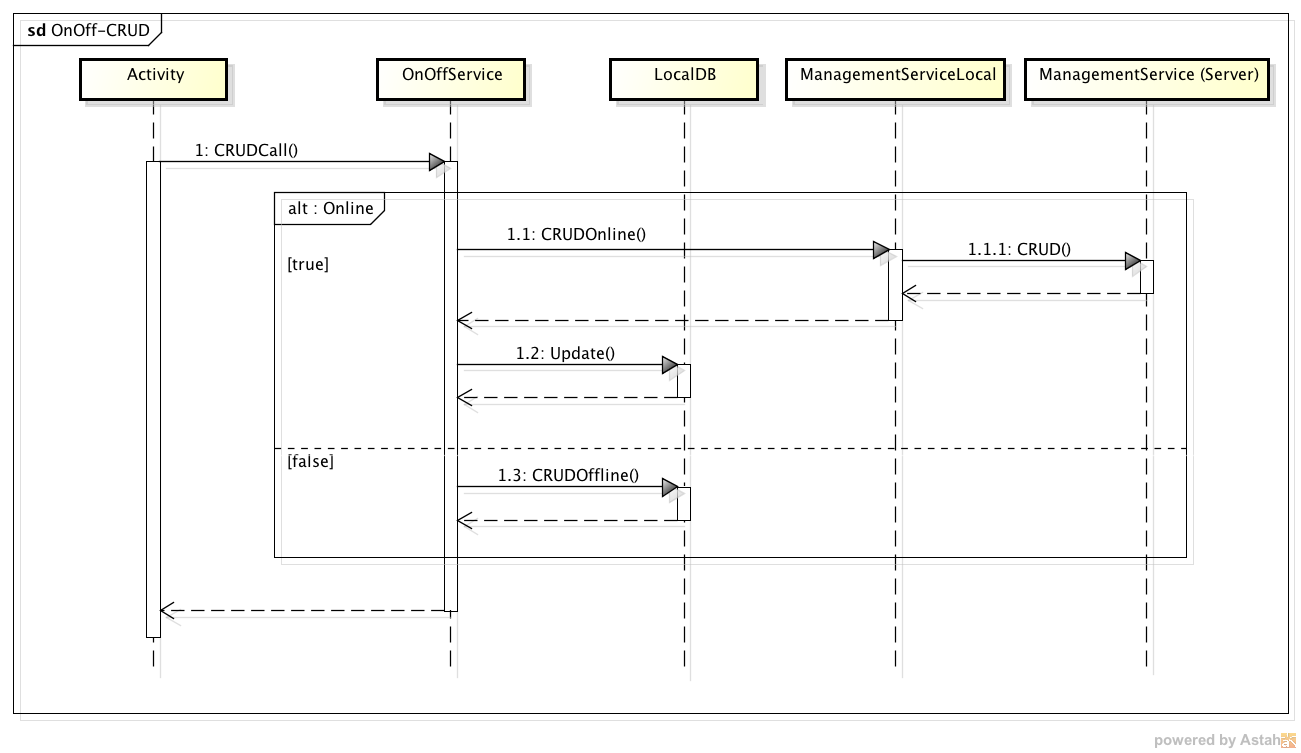
\includegraphics[width=\linewidth]{content/images/fITNat-OnOff-CRUD}
\caption{Sequenzdiagramm CRUD}
\label{pic:nat-CRUD}
\end{figure}
Die Hauptfunktionalität und -schwierigkeit lag in dem Szenario, dass die App gerade wieder eine Verbindung zum Server aufbaut und im Vorfeld Daten im Offline-Modus gespeichert hat, die dem Server noch nicht bekannt sind. Dieser Fall ist in dem Codeausschnitt \ref{lst:ConnectivityCheck} zu sehen. Dabei wird überprüft, ob die App in dem vorherigen Intervall noch im Offline-Modus war. 
\lstinputlisting[caption=Synchronisation der Offline-Daten, label=lst:Sync, style=sharpc]{content/listings/Sync.cs}
Ist dem so, wird in der lokalen Datenbank nach Trainings gesucht, die offline angelegt wurden. Diese werden dann mit dem Server abgeglichen und hochgeladen. Das Hochladen geschieht einzeln, damit im Fall eines abrupten Verbindungsverlustes maximal ein Datensatz verloren geht. Dabei wäre es möglich eine Transaktionsverwaltung für die Verbesserung zu integrieren, um dieses Problem zu verhindern. Bei dem Anlegen des Trainings fällt auf, dass die Attribute \textit{Username} und Passwort noch einmal übergeben werden. Diese Maßnahme musste ergriffen werden, um eine Verbindung zum Server herstellen zu können. Dazu wird eine \textit{Session} benötigt, die vorher noch nicht besteht, für den \textit{Upload} aber essentiell ist. Somit wird die \textit{Session} vor dem Hochladen abgerufen.
	\chapter{Realisierung der clientseitigen Implementierung als Webapplikation}
\label{cha:web-app}

\section{Definition einer Single Page Application}
\label{sec:Definition-SPA}

\section{AngularJs}
\label{sec:AngularJs}

\subsection{MVC}
\label{ssec:SPA-MVC}

\subsection{Services}
\label{ssec:SPA-Services}

\subsection{Promises}
\label{ssec:SPA-Promises}

\subsection{Routing}
\label{ssec:SPA-Routing}

\section{Umsetzung}
\label{sec:SPA-Umsetzung}

\subsection{Layout mit Twitter Bootstrap}
\label{ssec:SPA-twitter-bootstrap}

\begin{itemize}
\item Was ist das 
\item Vorteile: responsives Verhalten 
\end{itemize}

\subsection{Online-Check}
\label{ssec:Online-Check}

\subsection{Herausforderung statusloses Protokol Http}
\label{ssec:statusloses-http}

\begin{itemize}
\item Login
\end{itemize}

\section{CachedHttpService mit IndexedDB}
\label{sec:CachedHttpService}

\subsection{Exkurs IndexedDB}
\label{ssec:Exkurs-IndexedDB}

\subsection{Http-Verbs}
\label{ssec:Http-Verbs}

Umsetzung von Caching auf basis der Http-Verben statt einer konkreten implementierung für jede entity

\subsection{Synchronisation zwischen Server und SPA}
\label{ssec:Sync-SPA}

\section{Herausforderungen}
\label{sec:Herausforderungen-SPA}

\begin{itemize}
\item IndexedDB nicht voll implementiert
\item Code vollständig einsehbar: Probleme mit sensiblen Daten
\end{itemize}

	\chapter{Gegenüberstellung der clientseitigen Implementierungen}
\label{cha:gegenueberstellung}
Ziel dieses Kapitels ist die Gegenüberstellung der Erkenntnisse zur Entwicklung einer verlässlichen mobilen Applikation. Hierbei wird das neu erlangte Wissen zur Umsetzung einer Applikation als SPA und als native App bewertet, so dass mit der vorteilhafteren der beiden Optionen der Messeprototyp umgesetzt werden kann.

\section{Umsetzung als SPA}
\label{sec:gegenueberstellung-SPA}
Als erstes sollen die Vor- und Nachteile der Umsetzung des Clients als \textit{Single Page Application} aufgezeigt werden.

\subsection{Vorteile}
\label{sec:vorteile-SPA}
Bei der Umsetzung des Clients als Web Applikation zeigen sich die Vorteile besonders in der Umsetzung der Oberfläche. \\
Durch die Nutzung aktueller Web-Techniken und unter Nutzung geeigneter Frameworks lässt sich sehr leicht ein einheitliches Aussehen schaffen, welche für verschiedene Anzeigegrößen optimiert wurde. Hierbei ist man nicht nur auf mobile Endgeräte beschränkt sondern erhält quasi nebenbei eine Webseite, die bequem eine Desktop-Anwendung ersetzen kann. Auch die Umsetzung der Business-Logik konnte ohne großen Einarbeitung-Aufwand bewerkstelligt werden. Dabei fällt auf, dass durch das Voranschreiten von HTML5 viele Funktionen, welche vor einigen Jahren nur durch Desktop Applikationen umgesetzt werden, heute schon problemlos im Browser abbildbar sind. Hierbei zeigten sich aber auch die Schwächen einer Umsetzung als Web Applikation. 

\subsection{Nachteile}
\label{sec:nachteile-SPA}
Wie bereits erwähnt sind viele, aber noch nicht alle Techniken für den Browser umgesetzt. So ist die Umsetzung der \textit{IndexedDB} für iOS und Microsoft-Geräte noch sehr fehleranfällig\footcite{online:caniuse:indexedDB}. In diesem Punkt spiegelt sich auch das größte Problem jeder Web-Umsetzung wieder: Unterschiedliche Browser implementieren einige Apis anders oder teilweise auch gar nicht, sodass vieles der Entwicklungszeit für das Anpassen der Funktionen und Oberflächen für die verschiedenen Browser genutzt werden muss. Wenn es nun so ist, dass Kern-Komponenten wie in unserem Fall die IndexedDB in einigen wichtigen Browsern (iOS Safari-Nutzung bei 7.33\% (v. 8.1-8.4 Stand 31.08.2015\footcite{online:caniuse:indexedDB}) nicht ausreichen unterstützt werden, ist die Umsetzung dieses Teilaspekts für den produktiven Einsatz fast unmöglich. \\
Ein weiterer Nachteil ergibt sich aus der Nutzung von AngularJs. Da die gesamte Datenaufbereitung mit Authentifizierung und dem Routing auf Seiten des Clients passiert, können die lokal gespeicherten Daten mit Hilfe der Entwicklungswerkzeuge des Browsers einfach ausgelesen werden. Darum wäre es unter Sicherheitsaspekten fahrlässig, die hier vorgestellte Implementierung der Authentifizierung (siehe Kapitel \ref{ssec:statusloses-http}) ohne weitere Sicherheitsmaßnahmen produktiv zu stellen.

\section{Umsetzung als native App}
\label{sec:gegenueberstellung-native-app}

\subsection{Vorteile}
\label{sec:vorteile-native-app}

\subsection{Nachteile}
\label{sec:nachteile-native-app}

\section{Fazit: Weiterentwicklung als native App}
\label{sec:gegenueberstellung-fazit}

	\chapter{Fazit}
\label{fazit}
In diesem Kapitel wird eine Retrospektive des durchgeführten Projekts gegeben. Dabei wird zwischen dem Ergebnis bei der Erstellung der Applikationen und dem Erreichen der persönlichen Ziele unterschieden.
\section{Ziele / Ergebnisse}
\label{sec:ziele-ergebnisse}
Rückblickend kann das Projekt als ein Erfolg gesehen werden. \\
Aus dem Projekt ist eine umfassende Client-Server-Landschaft entstanden, welche die gesetzten Anforderungen an eine verlässliche mobile Applikation, sowohl in den Aspekten der Benutzerfreundlichkeit als auch der Verlässlichkeit, erfüllt. Sowohl der Server als auch beide Clients haben in den jeweils erstellten Meilensteine alle muss Kriterien erfüllt. Teilweise konnten sogar noch optionale Kann-Kriterien umgesetzt werden. So ist es beispielsweise möglich, sich an der Web \ac{API} zu registrieren oder in der nativen \gls{App} eine Trainingsstatistik aufzubauen. 
Dies ist besonders deshalb bemerkenswert, da die Projektteilnehmenden einen großteils der genutzten Techniken erst erlernen mussten. 
Alle im Projekt erzeugten Ressourcen können über das öffentliche Git-Repository unter \textit{\href{https://github.com/Fanuer/fIT}{https://github.com/Fanuer/fIT}} abgerufen werden. 

%Anfangs wurde ein Überblick über die Aufgabe gegeben und die Systemarchitektur vorgestellt. Darauf aufbauend wurden die verwendeten Technologien erörtert und die Umsetzungen der beiden Applikationen bis zu einem festgelegten Punkt dokumentiert. Die Implementierung des Servers wurde zusätzlich betrachtet. Die anschließende Gegenüberstellung der Apps hat ergeben, dass die Weiterentwicklung der Android-App in Hinsicht auf Sicherheit als einzige Lösung gesehen werden kann.\\
%Deshalb wurde für diese Applikation ein zweiter Meilenstein begonnen, um die Anforderungen an den umzusetzenden Prototypen zu implementieren. 
%Rückblickend kann das Projekt als ein großer Erfolg gesehen werden. Die eingangs formulierten Ziele konnten vollständig umgesetzt werden. Zudem wurden teilweise noch Funktionen umgesetzt, die über das formulierte Ziel hinaus gehen.\\
%Zusammenfassend ist es nun mit dem Prototypen möglich den kompletten Funktionsumfang der nativen Android-App auch im \textit{Oflline}-Modus nutzen zu können. 
\section{Erkenntnisse}
\label{sec:erkenntnisse}
Der Erkenntnisgewinn dieser Arbeit ist beträchtlich. \\
Es wurden vorwiegend unbekannte und für die Autoren neue Technologien verwendet. Die Einarbeitung geschah in den meisten Fällen reibungslos. Dies wurde gerade zu Anfang des Projekts jedoch auch als Risiko empfunden, welches ein Problem in der Umsetzung hätte verursachen können. Diese Zweifel waren jedoch im nach hinein unbegründet. \\
Die Tatsache, dass dieses Projekt von zwei Personen durchgeführt wurde, ergab sich als enormer Vorteil. Dies gestattet, punktuell Spezialwissen zu erwerben, was jeweils der anderen Person vermittelt werden musste. Dadurch wurde der Lerneffekt nochmals verstärkt und Zusammenhänge leichter vertieft.\\
Ebenfalls wurde von beiden Projektteilnehmer als sinnvoll erachtet, dass eine Komplettlösung für ein größeres Feld an Aufgaben, nämlich mobile Applikationen, geschaffen werden musste. Das meint, dass nicht nur einer Cache-Komponente für ein bestehendes System erstellt wurde, sondern jede Komponenten für die Realisierung der Systemlandschaft erstellt, verwaltet und veröffentlicht werden musste.\\
Somit konnte sich ein Einblick über alle anfallenden Arbeitsschritte zur Umsetzung einer mobilen Applikation geschaffen werden. 
\section{Ausblick}
\label{sec:ausblick}
Die Grundlage für den Ausbau dieses Projektes zu einer marktreifen \gls{App} ist gegeben. Der dahinter liegende Server ist stark genug, um eine größere Last an Anfragen zu bewältigen. Zum Ausbau dieses Projekts muss die \gls{Android}-\gls{App} weiterentwickelt werden. \\
Die Umsetzung aller wichtiger Funktionen wurde jeweils an mindestens einem Beispiel im Messeprototyp dargestellt und muss demnach nur noch auf die fehlenden Funktionalitäten übertragen werden.\\
Durch den nun tieferen Einblick in die Technologien sollte sich dieser Aufwand in Grenzen halten.\\
Auf Seiten dies Servers müssen hauptsächlich Sicherheitsfunktionen weiterentwickelt werden, um die Web API öffentlich nutzbar zumachen. Zu diesen Funktionen zählen beispielsweise die Validierung von ClientIDs, die Einschränkung eingehender Anfragen durch \ac{CORS} und die Signierung von Tokens. \\
Darüber hinaus kann eine Weiterentwicklung der \ac{App} dazu führen, dass die Web \ac{API} Ressourcen erweitert werden muss. 
	
	% ----------------- Ende des eigentlichen Textes
	

	%Verzeichnisse erstellen
	\chapter*{Glossar}
	\printglossaries	
  	\chapter*{Abkürzungsverzeichnis}
\addcontentsline{toc}{chapter}{Abkürzungsverzeichnis}  
\begin{acronym}[Visual Studio] %Längster Begriff
\setlength{\itemsep}{-\parsep}
	\acro{.apk}{Android Package}
	\acro{ACL}{Access Control Lists}
	\acro{AES}{Advanced Encryption Standard}
	\acro{AJAX}{Asynchronous JavaScript and XML}	
	\acro{ANR}{Application Not Responding}
	\acro{API}{Application Programming Interface}
	\acro{CORS}{Cross-origin resource sharing}
	\acro{CRUD}{Create Read Update Delete}	
	\acro{CSS}{Cascading Style Sheet}
	\acro{DLL}{Dynamic Link Library}
	\acro{DRAM}{Dynamischer \ac{RAM}}
	\acro{HTML}{Hypertext Markup Language}	
	\acro{HTTP}{Hypertext Transfer Protocol}	
	\acro{HTTPS}{Hyper Text Transfer Protocol Secure}	
	\acro{IDE}{Integrated Development Environment}
	\acro{JSON}{JavaScript Object Notation}	
	\acro{JWT}{\ac{JSON} Web Token}	
	\acro{MSSQL}{Microsoft SQL Server}
	\acro{MVC}{Model-View-Controller}	
	\acro{MVVM}{Model-View-ViewModel}
	\acro{OR-Mapper}{objekt-relationaler Mapper}
	\acro{PCL}{Portable Class Library}
	\acro{RAM}{Random Access Memory}
	\acro{RBAC}{Role Based Access Control}	
	\acro{REST}{Representational State Transfer}	
	\acro{SPA}{Single Page Application}
	\acro{SRAM}{Statischer \ac{RAM}}
	\acro{TCP}{Transmission Control Protocol}
	\acro{URI}{Uniform Resource Identifier}		
	\acro{URL}{Uniform Resource Locator}		
	\acro{Visual Studio}{Microsoft Visual Studio 2015 Community Edition}		
	\acro{VM}{Virtuelle Maschine}
	\acro{Web-App}{mobil-optimierte Webseite}
	\acro{XML}{Extensible Markup Language}
\end{acronym}

	\listoffigures
	\listoftables
	\lstlistoflistings
	
	\appendix
	\nocite{*} 


	%Literaturverzeichnis erstellen
	\bibliography{bib/bib}
	\bibliographystyle{jurabib}

	
	%\chapter{Anhang}
\label{cha:anhang}

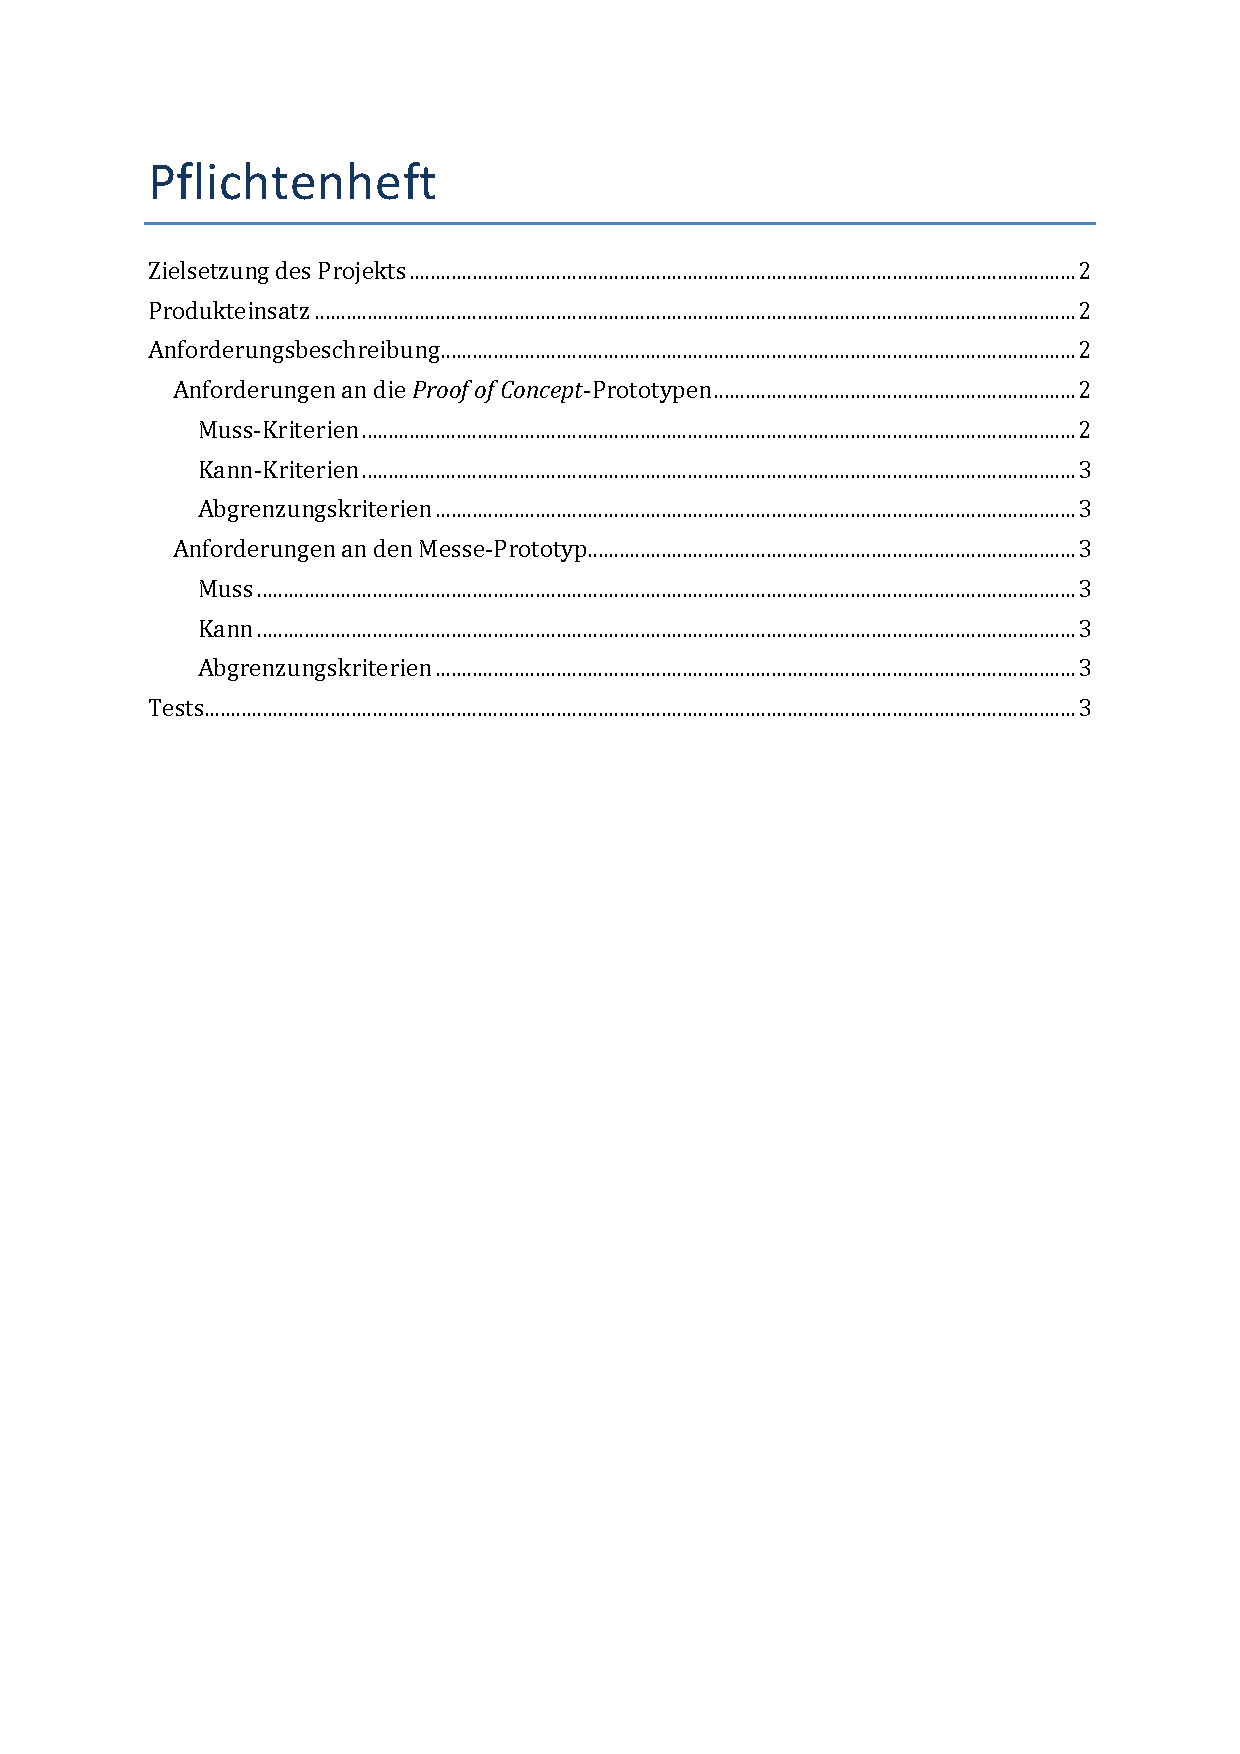
\includepdf[pages={-},frame= true, scale=0.68, pagecommand=\section{Pflichtenheft}\label{sec:Pflichtenheft}]{content/additional/Pflichtenheft.pdf}

\section{Cache Post}
\label{sec:cachePost}

%CachePush-Bild
\begin{figure}[!h]
\centering
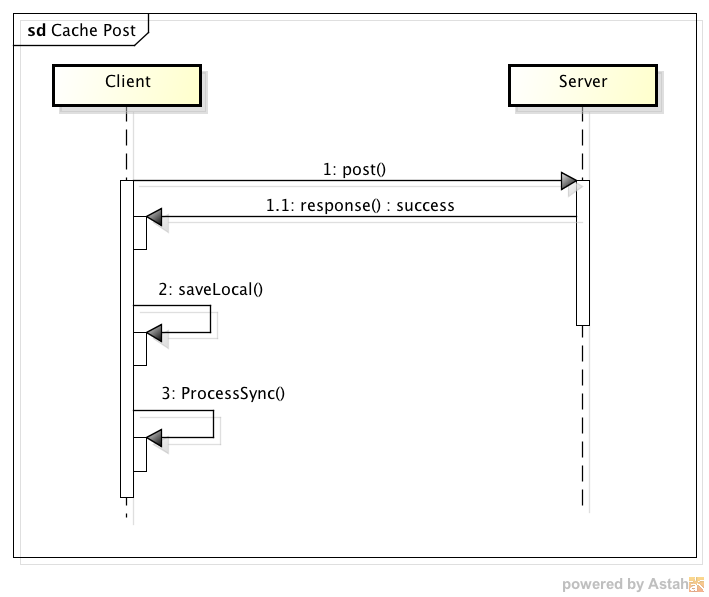
\includegraphics[width=0.8\linewidth]{content/images/Cache-Post}
\caption{Hochladen zum Server}
\label{pic:cachePost}
\end{figure}

\section{User-Story in der nativen App}
\label{sec:UserStory}
%Startseite
\begin{figure}[!h]
\centering
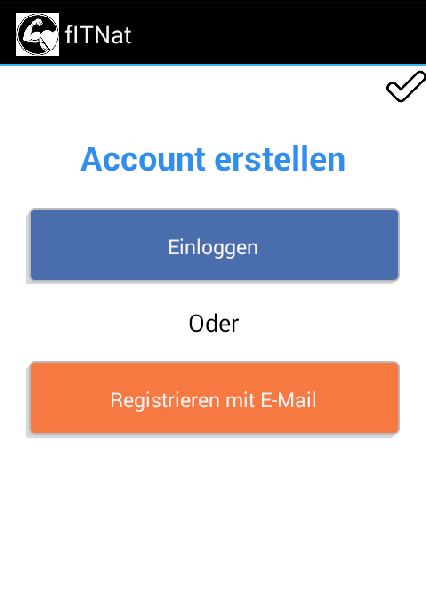
\includegraphics[width=0.5\linewidth]{content/images/App/Startseite}
\caption{Startseite}
\label{pic:natAppStartseite}
\end{figure}
%Login
\begin{figure}[!h]
\centering
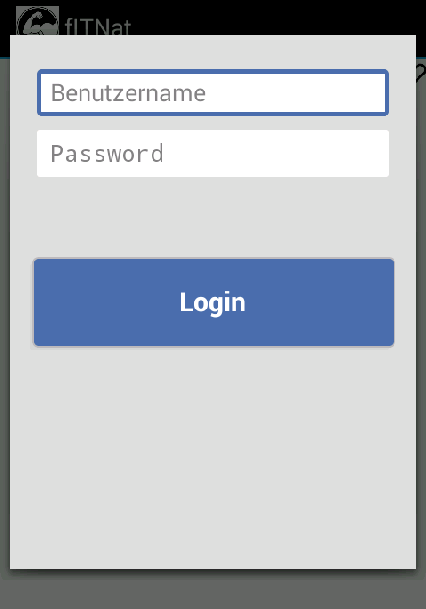
\includegraphics[width=0.5\linewidth]{content/images/App/SignIn}
\caption{Login}
\label{pic:natAppLogin}
\end{figure}
%Reistrierung
\begin{figure}[!h]
\centering
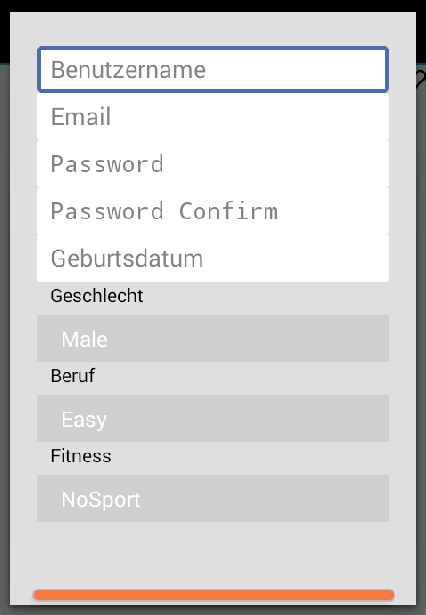
\includegraphics[width=0.5\linewidth]{content/images/App/SignUp}
\caption{Registrierung}
\label{pic:natAppRegistrierung}
\end{figure}
%Trainingspläne
\begin{figure}[!h]
\centering
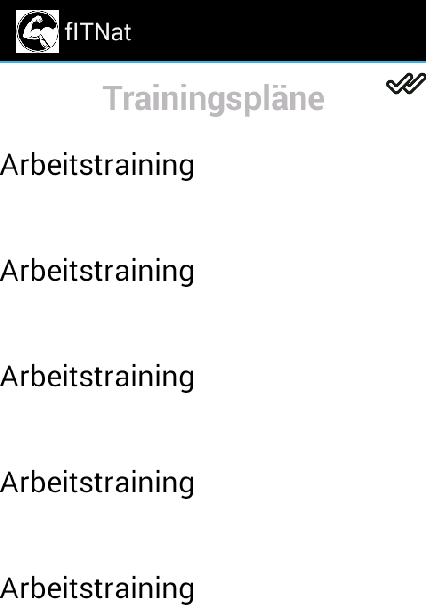
\includegraphics[width=0.5\linewidth]{content/images/App/Trainingsplan}
\caption{Übersicht der Trainingspläne}
\label{pic:natAppTrainingspläne}
\end{figure}
%Übungen
\begin{figure}[!h]
\centering
\includegraphics[width=0.5\linewidth]{content/images/App/Übungen}
\caption{Übersicht der Übungen}
\label{pic:natAppÜbungen}
\end{figure}
%Training
\begin{figure}[!h]
\centering
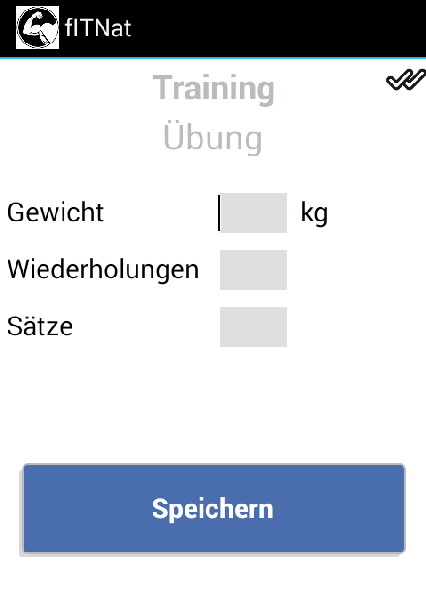
\includegraphics[width=0.5\linewidth]{content/images/App/Training}
\caption{Training}
\label{pic:natAppTraining}
\end{figure}
%Statistik
\begin{figure}[!h]
\centering
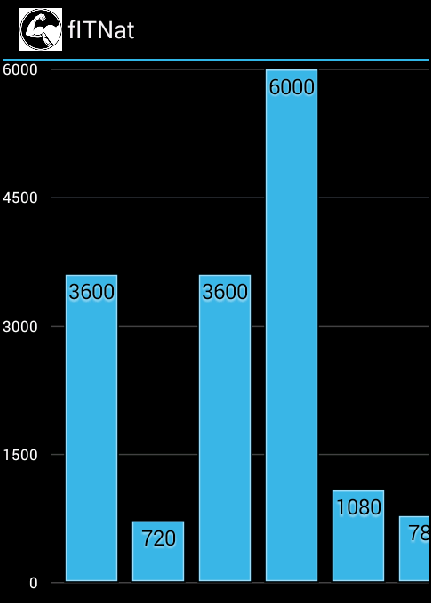
\includegraphics[width=0.5\linewidth]{content/images/App/Statistik}
\caption{Statistik}
\label{pic:natAppStatistik}
\end{figure}

\section{Funktionsumfang}
\label{natAppFunktionen}
	\chapter{Eidesstattliche Erkl�rung}
Gem�� �\,17,(5) der BPO erkl�re ich an Eides statt, dass ich die vorliegende Arbeit
selbst�ndig angefertigt habe. Ich habe mich keiner fremden Hilfe bedient und keine
anderen, als die angegebenen Quellen und Hilfsmittel benutzt. Alle Stellen, die
w�rtlich oder sinngem�� ver�ffentlichten oder nicht ver�ffentlichten Schriften und
anderen Quellen entnommen sind, habe ich als solche kenntlich gemacht. Diese
Arbeit hat in gleicher oder �hnlicher Form noch keiner Pr�fungsbeh�rde vorgelegen.
\vspace{3\baselineskip}\\
Dortmund, \thedate \hfill \theauthor

\vspace{1cm}
\section*{Erkl�rung}
Mir ist bekannt, dass nach �\,156~StGB bzw. �\,163~StGB eine falsche Versicherung
an Eides Statt bzw. eine fahrl�ssige falsche Versicherung an Eides Statt mit
Freiheitsstrafe bis zu drei Jahren bzw. bis zu einem Jahr oder mit Geldstrafe
bestraft werden kann.
\vspace{3\baselineskip}\\
Dortmund, \thedate \hfill \theauthor

\end{document}
